\section{Analysis of Previous Design}\label{sec:prev-design-analysis}
To test the hypothesised issue with the previous design, animations of the 2D simulation were generated, and the change in mass of the solid phase was recorded.~\autoref{fig:old-design-phase-density} shows a snapshot at two seconds into the transient simulation. 
\begin{figure}[htbp]
    \centering
    
    \begin{minipage}{0.4\textwidth}
        \centering
        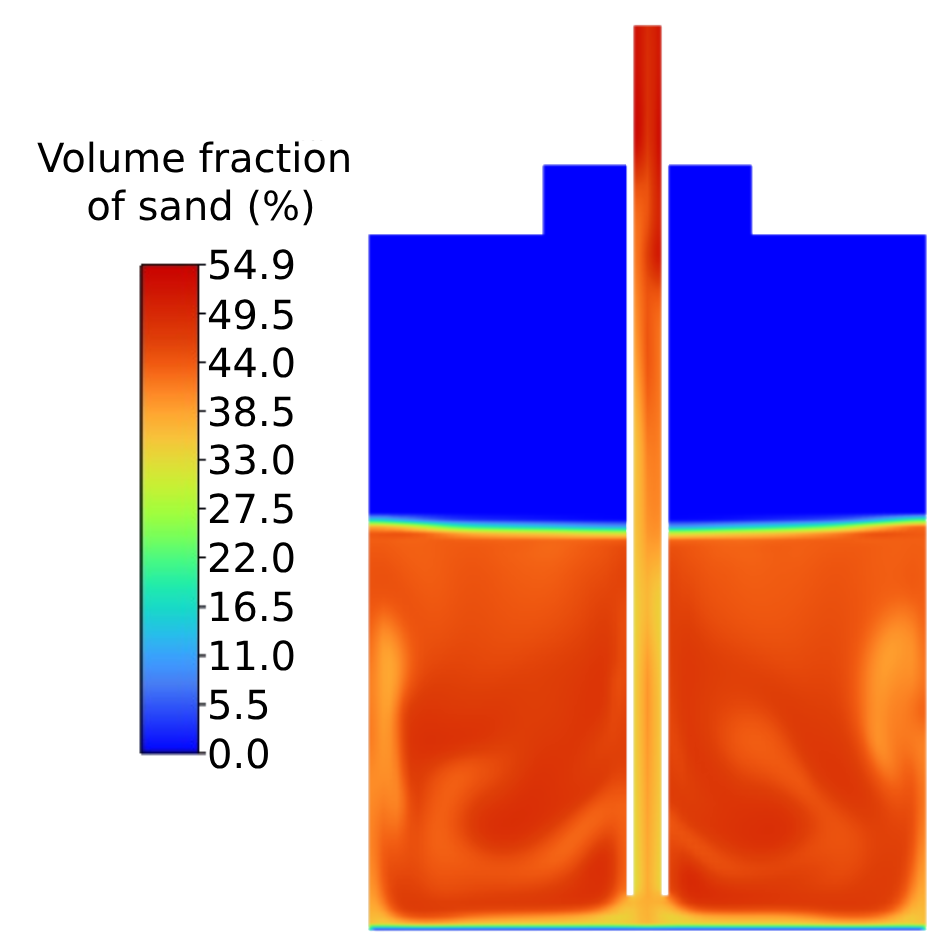
\includegraphics[width=\textwidth]{../report_assets/grav_better.png}
        \caption*{(a) Under Earth's Gravity}
    \end{minipage}
    \hfill
    \begin{minipage}{0.4\textwidth}
        \centering
        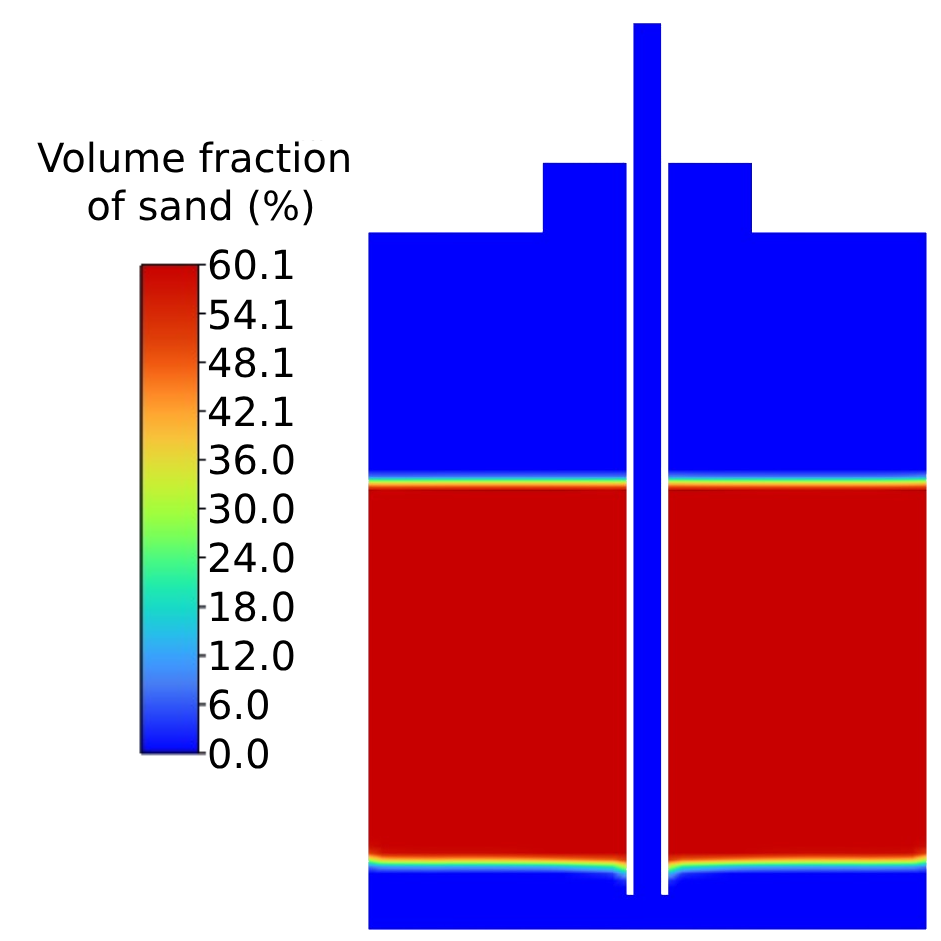
\includegraphics[width=\textwidth]{../report_assets/no_grav_better.png}
        \caption*{(b) Under Microgravity}
    \end{minipage}
    \caption{Phase Density of Old Design after 2 Seconds}\label{fig:old-design-phase-density}
\end{figure}
As illustrated, there is a marked difference in the powder distribution between the two cases. While the powder in the tank under gravity appears to fully fluidise, the tank in mircogravity remains relatively unaffected by the flow. This is likely because the steady-state flow field does not interact with the region of the tank where the powder settles. For completeness, all unprocessed simulation images are provided in \autoref{sec:unprocessed-images}.

\begin{figure}[htbp]
    \centering
    
    \begin{minipage}{0.54\textwidth}
        \centering
        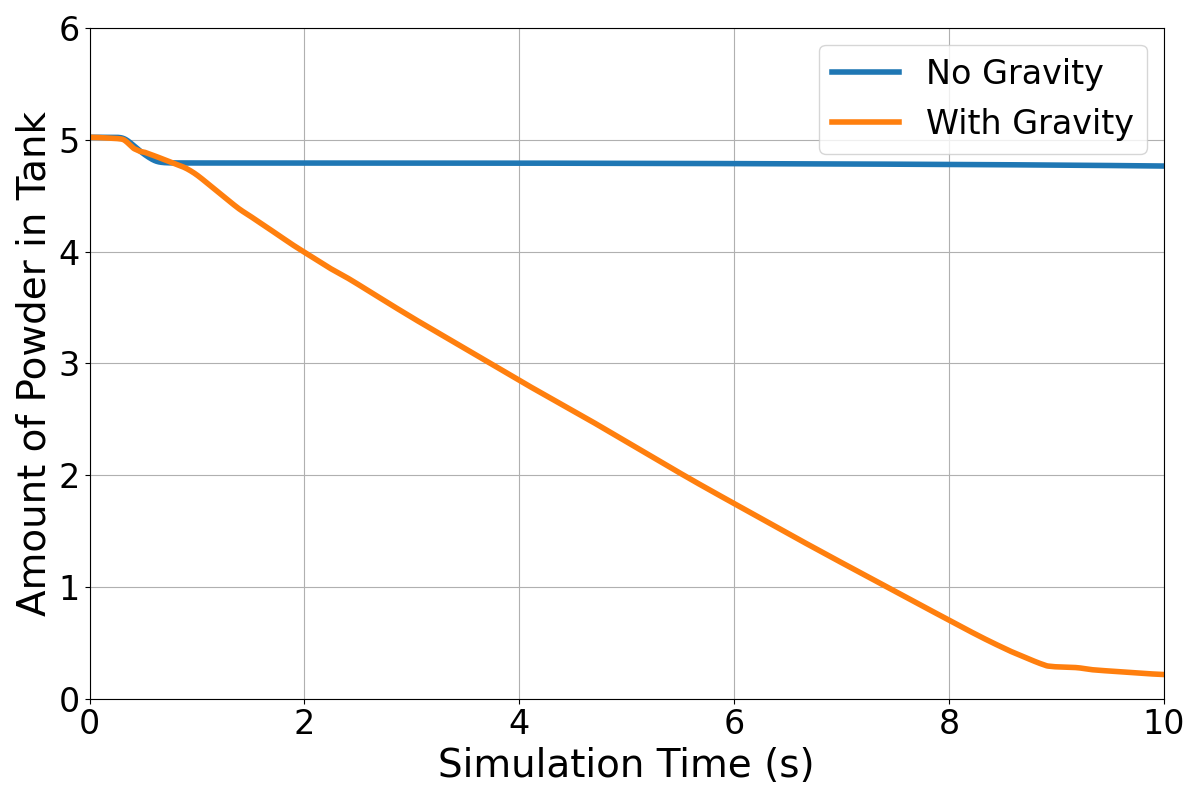
\includegraphics[width=\textwidth]{../report_assets/old_design_out.png}
        \caption{Change of Mass in the Tank Over Time}\label{fig:old-design-mass-change}
    \end{minipage}
    \hfill
    \begin{minipage}{0.4\textwidth}
        \centering
        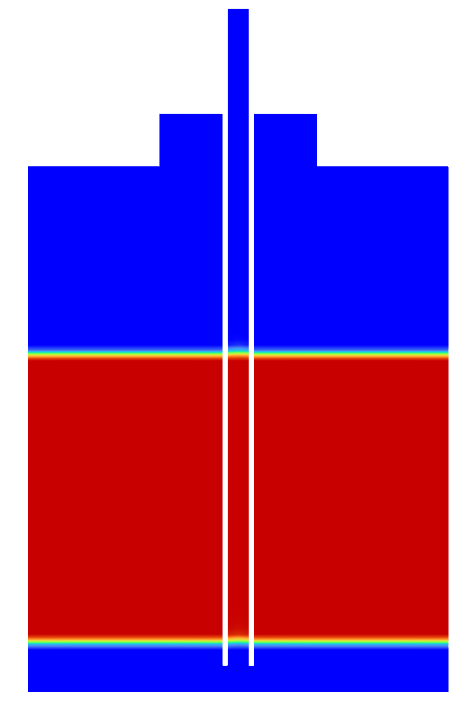
\includegraphics[width=0.6\textwidth]{../report_assets/old_initial.png}
        \caption{Initial Powder Configuration}\label{fig:old-initial}
    \end{minipage}
\end{figure}
\autoref{fig:old-design-mass-change} presents the change in amount of powder within the tank over time, measured by integrating the volume fraction of the solid phase over the entire geometry. At roughly 0.5 seconds, both simulations exhibit a noticeable drop in powder content. This behaviour is attributed to the initial conditions of the simulation, as shown in \autoref{fig:old-initial}, where the powder was initially located within the pipe and was rapidly expelled from the system. Beyond this point, a significant divergence in powder dispensing rates emerges between the two cases, further supporting the hypothesis that the previous design is less suitable for microgravity applications and justifying the decision to redesign the tank. 

As mentioned in \autoref{sec:old-design-method}, this analysis was conducted with a relatively coarse mesh, which may have influenced the accuracy of the results. The primary concerns are the potential under-resolution of key flow gradients and inaccuracies in the momentum exchange between the two phases. However, given the simplicity of the geometry and the low inlet velocity, it is assumed that any impact from insufficient resolution of velocity or pressure gradients is minimal. The effect on momentum exchange is less certain and was considered acceptable based on the author's understanding of the expected system behavior. With additional time, this area should be explored further through a mesh convergence study to validate these preliminary findings.

Another area for improvement involves the inlet boundary condition. A pressure inlet would more accurately represent the physical system, but due to limitations in the simulation software, there was no straightforward method to prevent powder from exiting through this inlet if it were modelled that way. This issue could be addressed using a user-defined function (UDF). By first simulating the system with a pressure inlet and no powder, the resulting inlet velocity profile could be extracted and then applied to the current analysis using a UDF.\@

\section{Analysis and Testing Tank Design}\label{sec:pressure-testing}
As mentioned in \autoref{sec:tank-fea-setup}, validation of the tank design was conducted in two stages: first through FEA and hand calculations prior to manufacturing, and then through hydrostatic pressure testing of the completed tank.

The initial FEA was performed using a configuration with six bolt holes. However, this was increased to eight after the predicted stress in the six-bolt configuration exceeded the yield strength of acrylic. As seen in \autoref{fig:fea-results}, the eight-bolt hole configuration shows stresses that are close to, but still below, the material's yield strength.
\begin{figure}[htbp]
    \centering

    \begin{minipage}{0.45\textwidth}
        \centering
        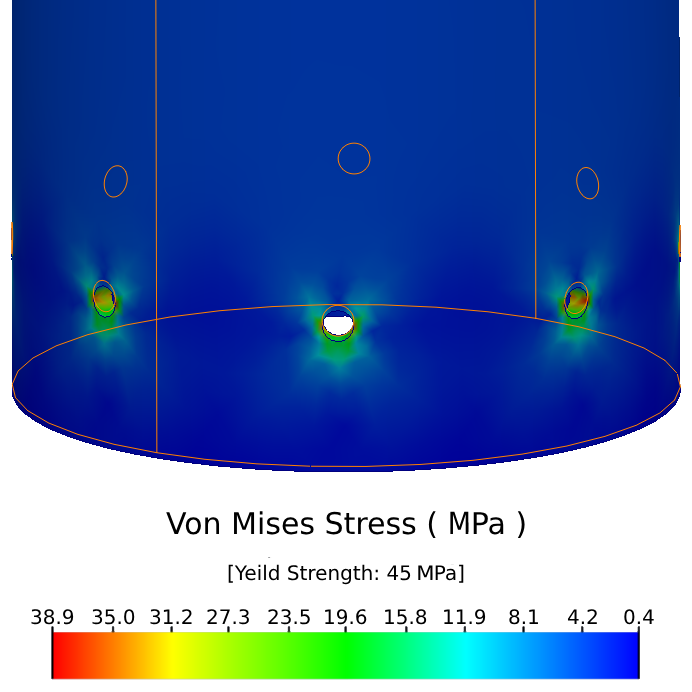
\includegraphics[width=\textwidth]{../report_assets/fine_mesh_results.png}
        \caption*{(a) Fine Mesh}
    \end{minipage}    
    \hfill
    \begin{minipage}{0.45\textwidth}
        \centering
        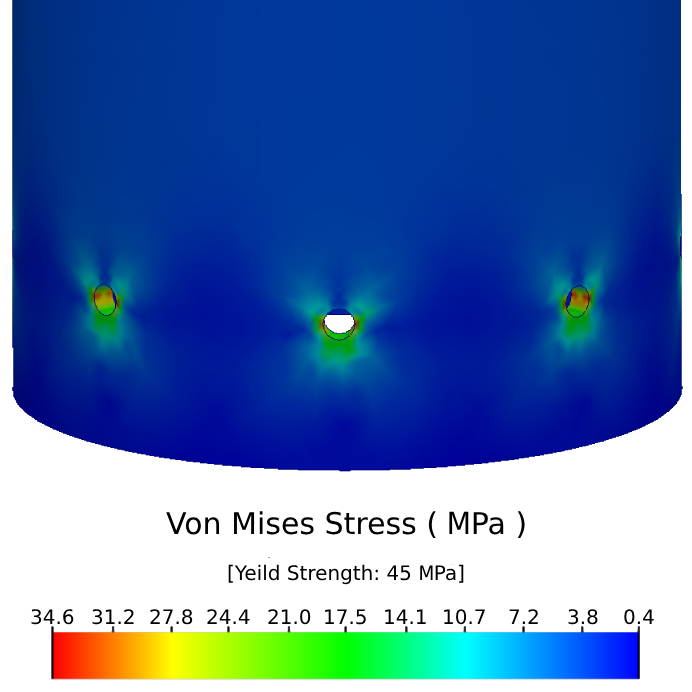
\includegraphics[width=\textwidth]{../report_assets/coarse_mesh_results.png}
        \caption*{(b) More Coarse Mesh}
    \end{minipage}    
    \caption{Stress Concentrations Around Tank Bolt Holes}\label{fig:fea-results}

\end{figure}  
\autoref{fig:fea-results} (a) shows the original vertices of the tank under no load, overlaid in orange on the deformed tank geometry. As the difference between the undeformed and deformed shapes is minimal, nonlinear deformation effects were considered negligible. Cylindrical geometries are inherently resistant to buckling, especially when pressurised internally, so buckling was not investigated in detail.

While a slight increase in von Mises stress was observed in the finer mesh, this was attributed to improved resolution at the boundary between the loaded and unloaded surfaces of the bolt holes. Since the real load application does not exactly match the simplified simulation boundary condition, the observed stress concentrations were deemed acceptable to start manufacturing.

The next failure mode checked was hoop stress rupture, evaluated using Lamé's equations. These calculations yielded a maximum stress of 8.88 MPa at the inner wall and 8.18 MPa at the outer wall. As these values are significantly lower than the stress concentrations around the bolt holes, hoop stress rupture was not considered the critical failure mode.

After manufacturing, the tank underwent hydrostatic pressure testing. During the first attempt, pressurising the tank with water caused the epoxy-Delrin interface to separate. Although this failure mode was anticipated during the design phase, it was expected that reattaching the end cap using a more plastic-compatible epoxy, along with thorough surface preperation of the Delrin bonding area, would resolve the issue. This assumption was validated in the subsequent pressure test, shown in \autoref{fig:hydro-results}.
\begin{figure}[htbp]
    \centering

    \begin{minipage}{0.45\textwidth}
        \centering
        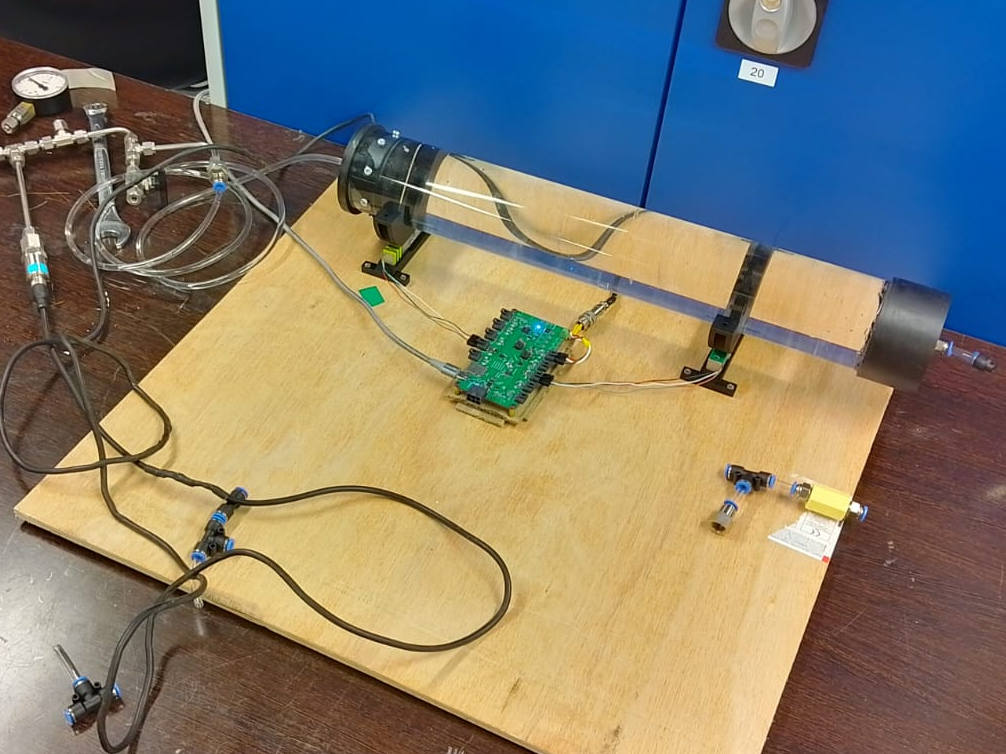
\includegraphics[width=\textwidth]{../report_assets/hydro_testing_setup.png}
        \caption*{(a) Hydrostatic Pressure Testing Setup}
    \end{minipage}    
    \hfill
    \begin{minipage}{0.45\textwidth}
        \centering
        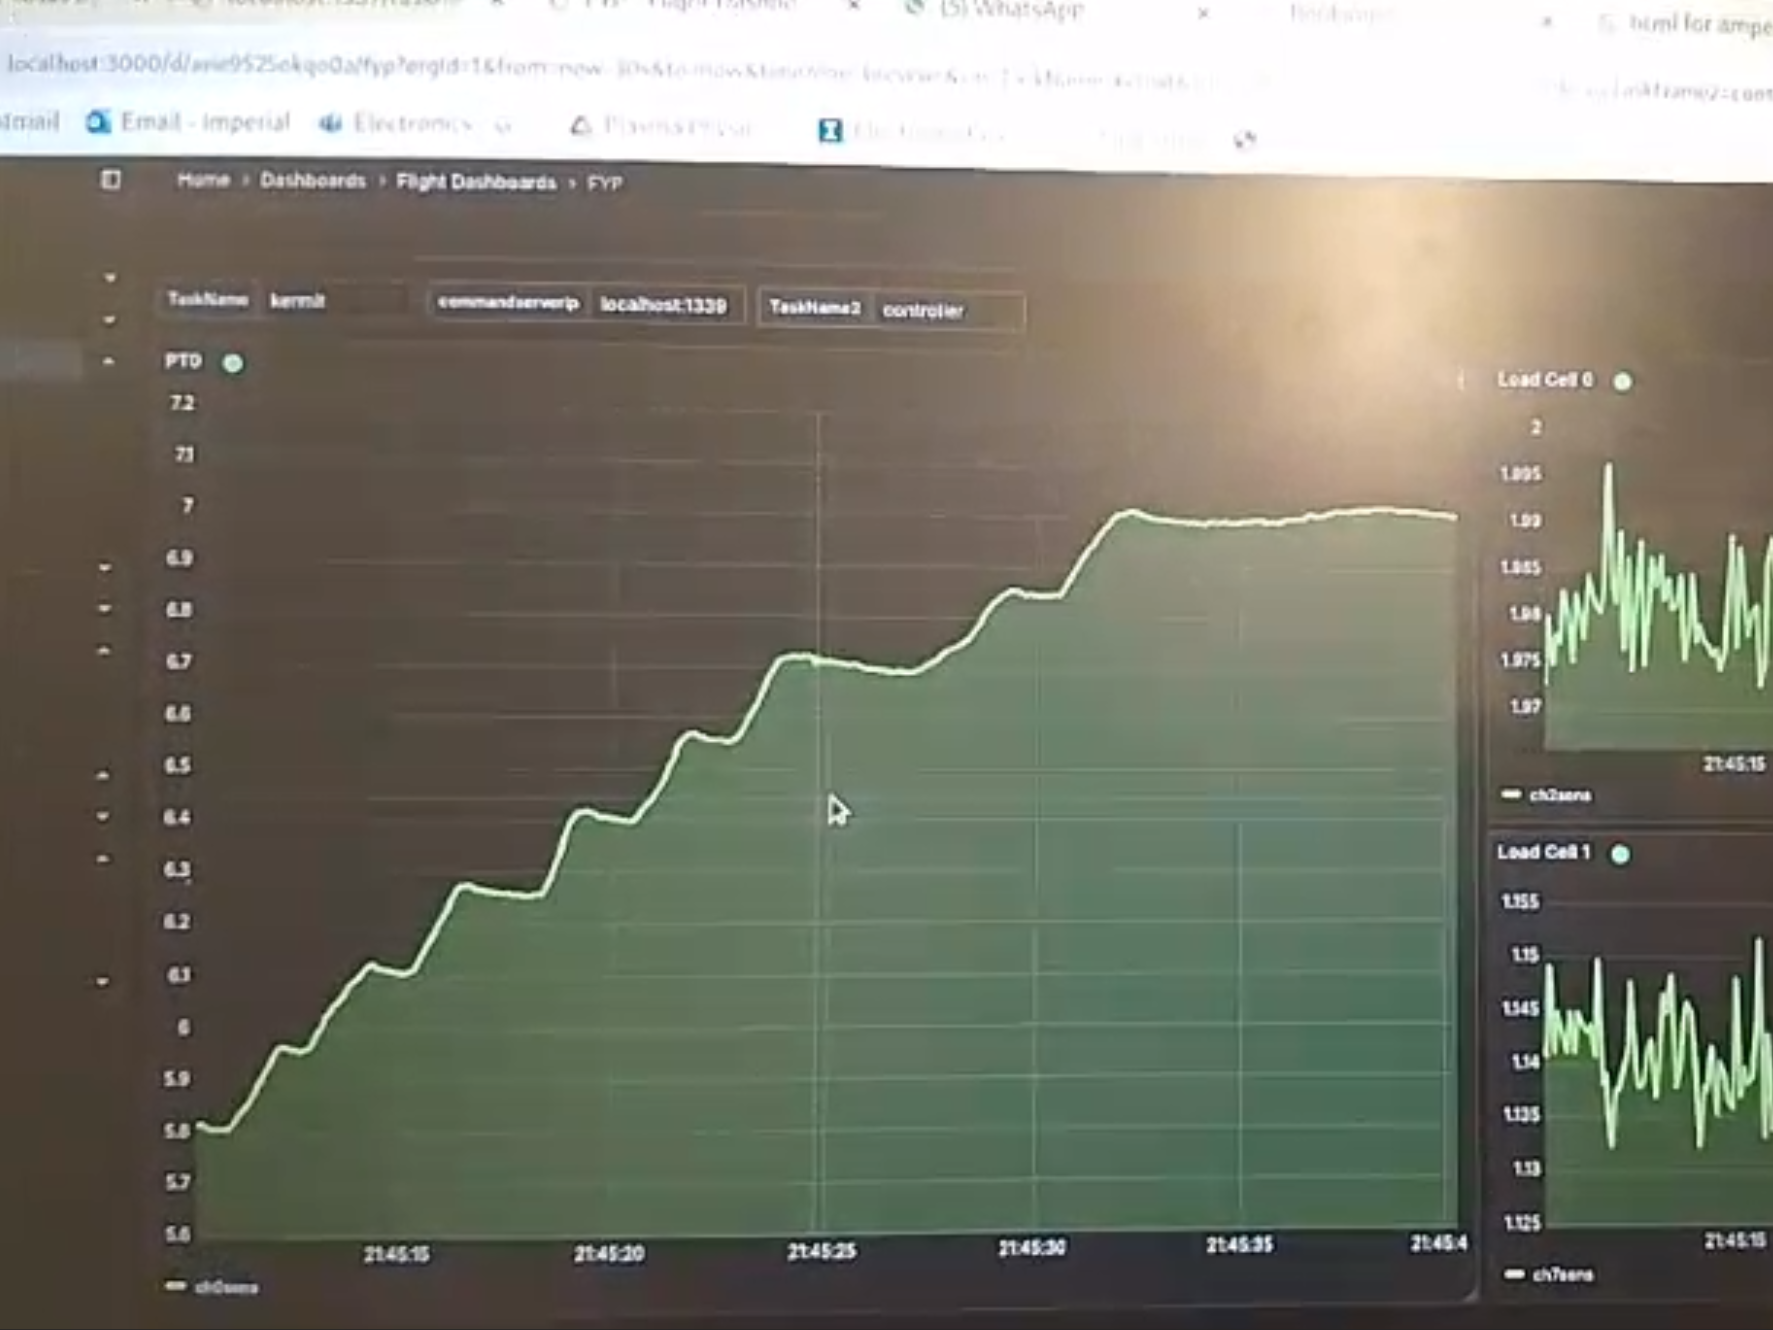
\includegraphics[width=\textwidth]{../report_assets/hydro_grafana.png}
        \caption*{(b) Screenshot of Results from Video}
    \end{minipage}    
    \caption{Hydrostatic Pressure Testing of Tank}\label{fig:hydro-results}

\end{figure}  
Unfortunately, only a video recording of the test was taken and the logged pressure data was not captured. A screenshot of the video is shown in \autoref{fig:hydro-results} (b), where the jagged rise in gauge pressure is from the manual actuation of the pump. The tank held successfully held a gauge pressure of 7 bar for approximately 2 to 3 minutes before the pressure was released. Although maintaining pressure for a longer durations would have provided greater confidence in the tank's safety, formal pressure vessel certification was not required for the intended experimental use and was therefore not pursued.

\section{First Test}\label{sec:first-test}
As mentioned in \autoref{sec:piston}, the initial test was conducted without sand and failed to push the piston down the tank. This quick test motivated the need to characterise the pressure source, as the pressure readings upstream and downstream of the tank were both lower and more sluggish than expected. As a result the failure mode of piston crumpling was ruled out, and subsequent piston designs did not account for this possibility. Following the characterisation of the pressure source, the second piston was tested, seen in \autoref{fig:first-test}. 

\begin{figure}[htbp]
    \centering
    
    \begin{minipage}{0.6\textwidth}
        \centering
        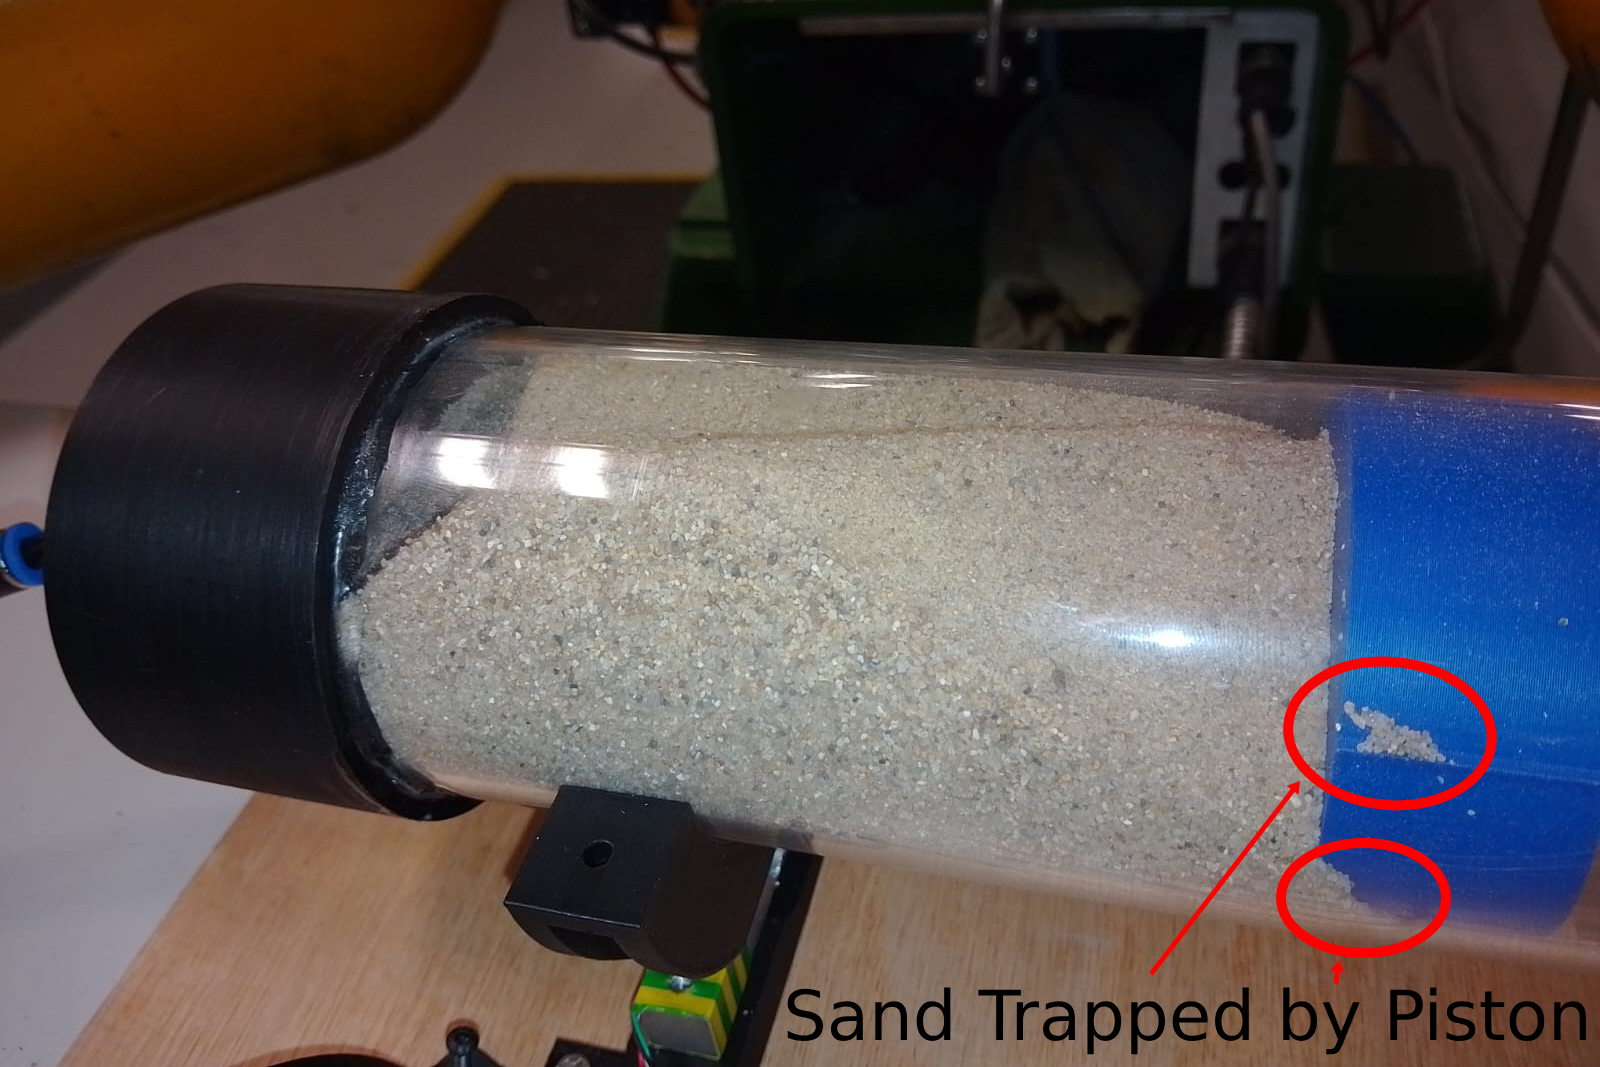
\includegraphics[width=\textwidth]{../report_assets/first_test.png}
        \caption{Result of First Powder Test}\label{fig:first-test}
    \end{minipage}
    
\end{figure}
The piston initially started near the inlet of the tank and was successfully pushed toward the outlet. However, upon reaching the sand, it became stuck. The unpacked grains formed a wedge beneath the piston, causing it to jam against the tank walls. Since the powder was not compacted against the outlet, ratholing occurred, with gas entraining sand particles through the outlet—highlighting an undesirable dispensing regime.

The piston-to-wall clearance was designed to be 1 mm, the same order of magnitude as the diameter of some of the large grains of sand, so it is expected that this specific issue would not have occurred with finer-grain sand. While options such as purchasing finer sand or crushing the current sample were considered, it was ultimately decided to pursue a new design. This jamming behavior is not well reported in piston tank design literature and posed challenges for friction characterisation. Although a full analysis of the piston mechanics was of great interest, complexities in the underlying physics pushed it outside the scope of the project due to time constraints.

\section{Characterising Pressure Source}\label{sec:static_test}
\subsection{Initial Test}
The first step in characterising the system was to investigate the static pressure losses within the tank in the absence of a piston or any powder. This immediately revealed an issue: the static pressure readings, assuming a gas source with a stagnation pressure of 4 to 6 bar, were significantly lower than expected, as shown in~\autoref{fig:static-pressure-drop}.
\begin{figure}[htbp]
    \centering

    \begin{minipage}{0.45\textwidth}
        \centering
        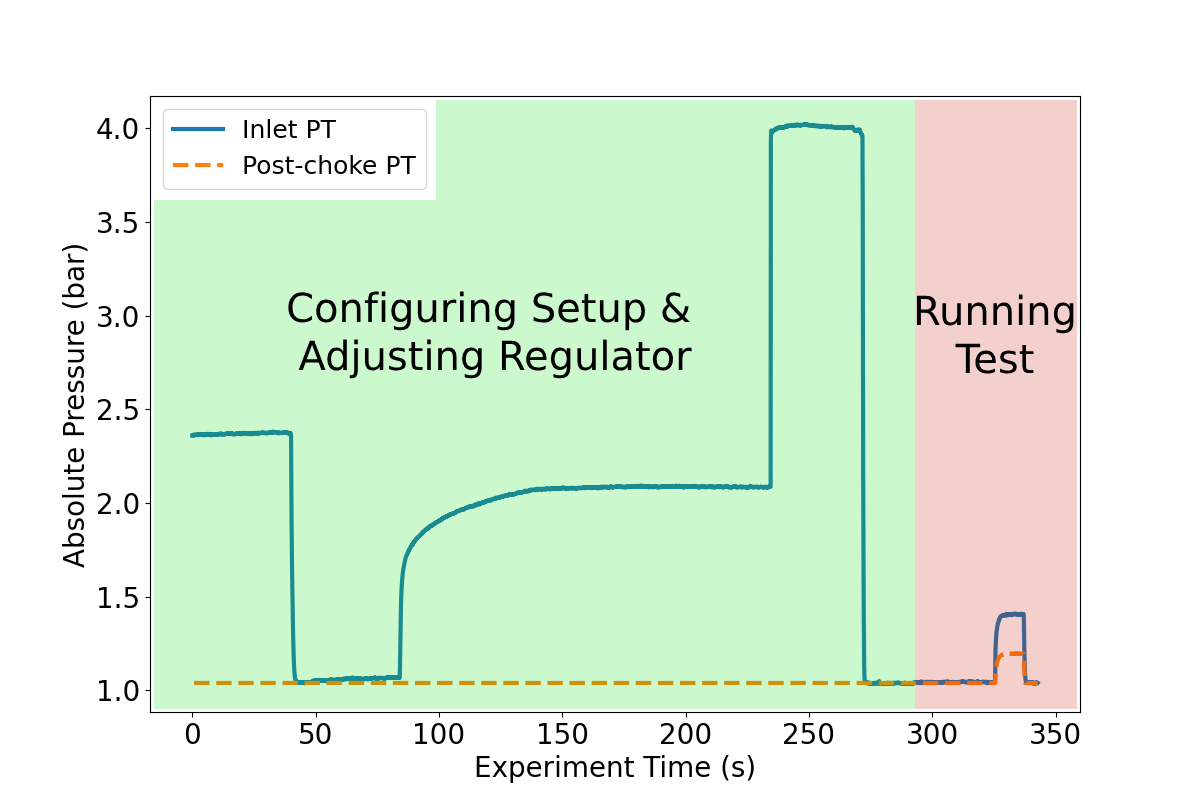
\includegraphics[width=\textwidth]{../report_assets/3_bar_static_full.png}
        \caption*{(a) Full Dataset from 4 bar Test}
    \end{minipage}    
    \hfill
    \begin{minipage}{0.45\textwidth}
        \centering
        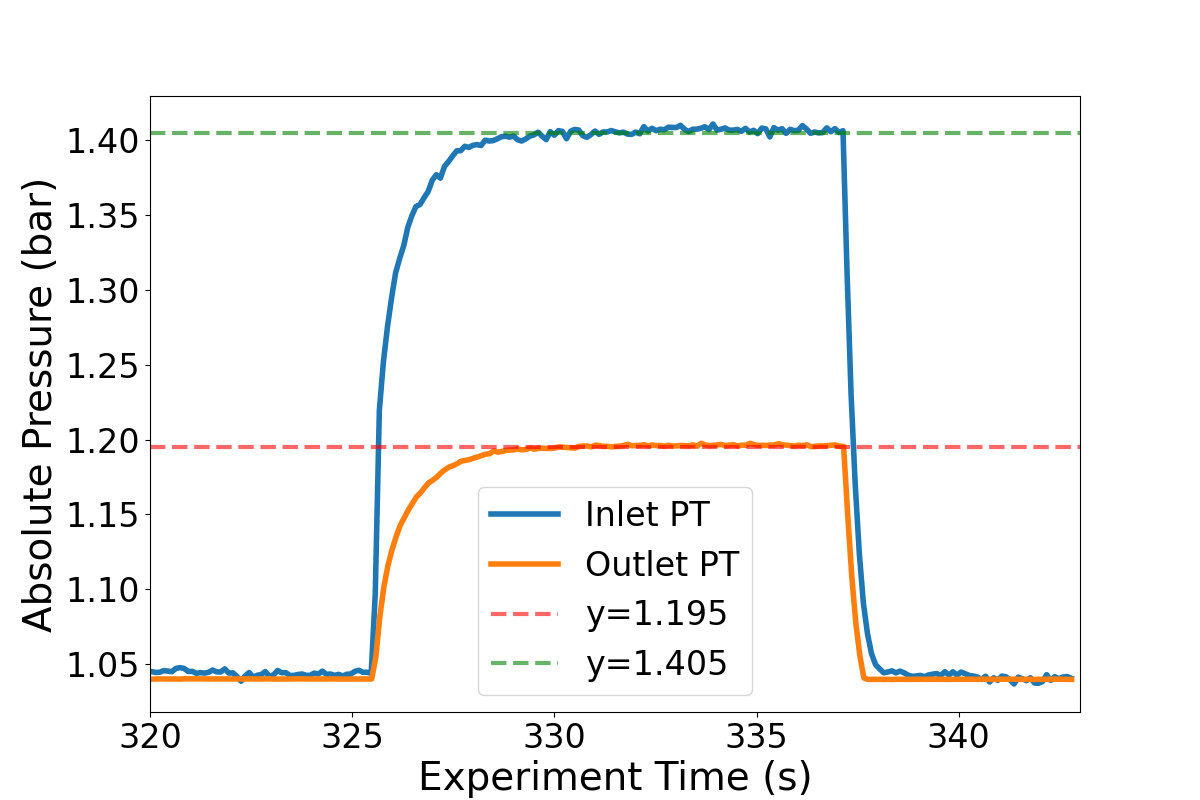
\includegraphics[width=\textwidth]{../report_assets/3_bar_static.png}
        \caption*{(b) Static Pressure from 4 bar}
    \end{minipage}    
    \begin{minipage}{0.45\textwidth}
        \centering
        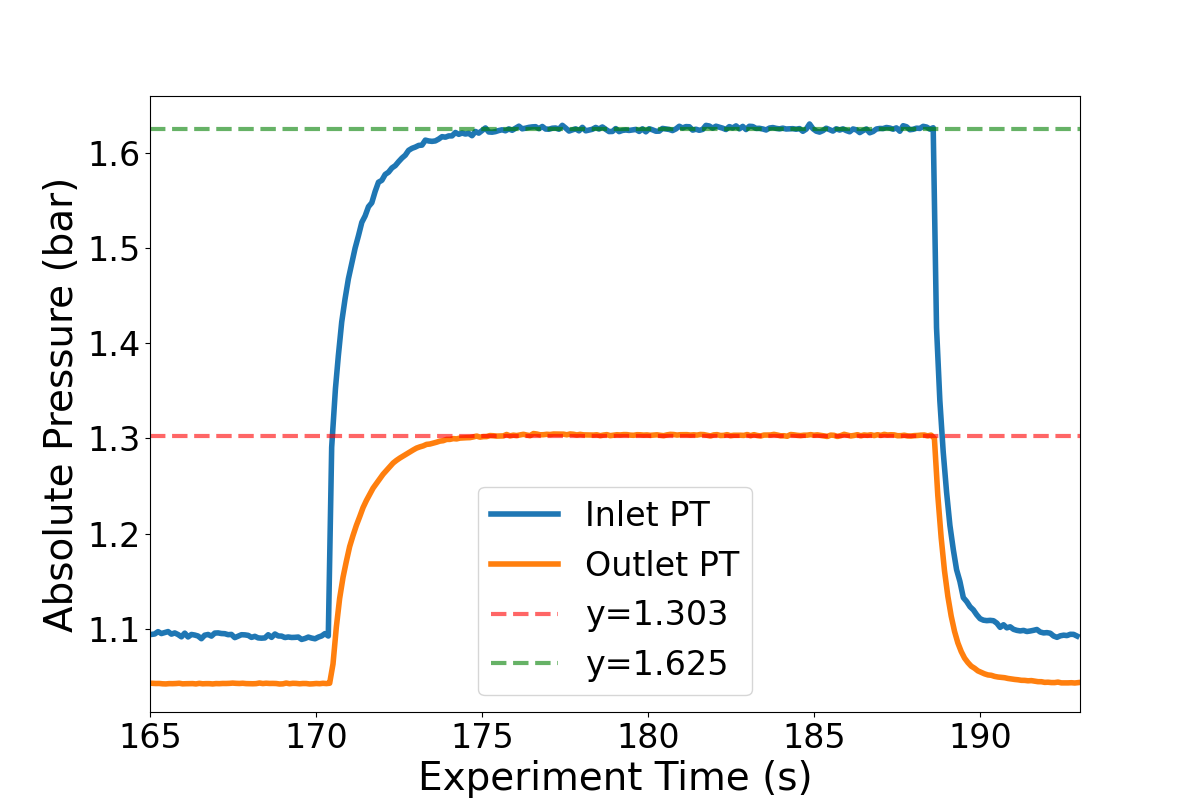
\includegraphics[width=\textwidth]{../report_assets/4_bar_static.png}
        \caption*{(c) Static Pressure from 5 bar}
    \end{minipage}    
    \hfill
    \begin{minipage}{0.45\textwidth}
        \centering
        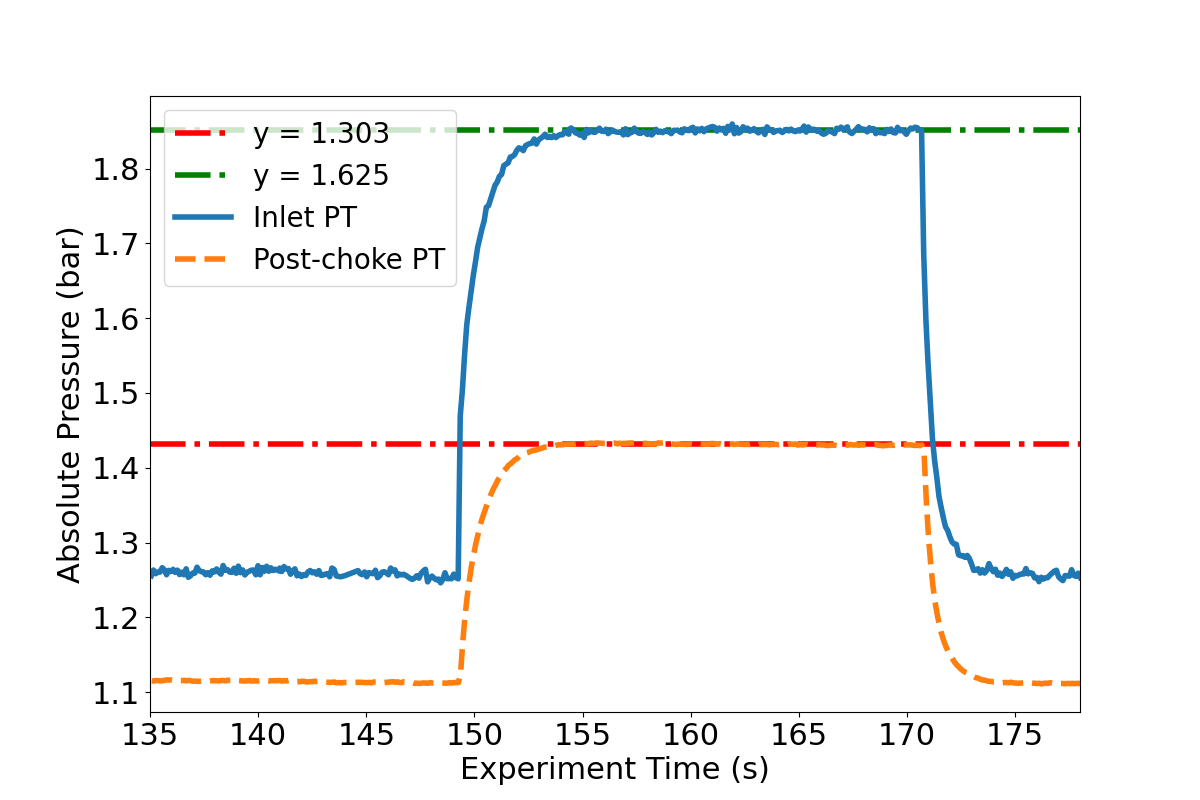
\includegraphics[width=\textwidth]{../report_assets/5_bar_static.png}
        \caption*{(d) Static Pressure from 6 bar}
    \end{minipage}    

    \caption{Static Pressure Readings Before and After the Tank at Different Pressures}\label{fig:static-pressure-drop}
\end{figure}    
If the compressed air line were truly supplying a stagnation pressure of 4 bar, isentropic flow relations suggest that the flow would have a Mach number of approximately 1.3, an unlikely result under the given conditions.

As shown in \autoref{fig:static-pressure-drop} (a), the regulator was capable of maintaining a static pressure of 4 bar when the system was closed. Upon opening the system, one might expect the regulator to continue maintaining this 4 bar pressure, with only moderate reductions caused by static pressure losses and flow acceleration downstream of the regulator. However, by the time the flow reached the pressure transducer upstream of the tank, the static pressure had fallen to 1.4 bar.

\subsection{Further Investigation}
In an attempt to diagnose this behaviour, follow-up tests were conducted with different setups and a 4 bar inlet pressure to validate a component of the system was not to blame. As seen in \autoref{fig:follow-up-stat-test}, the performance with the additional regulator or removal of the solenoid valve was much worse giving even lower static pressure readings. 
\begin{figure}[htbp]
    \centering

    \begin{minipage}{0.45\textwidth}
        \centering
        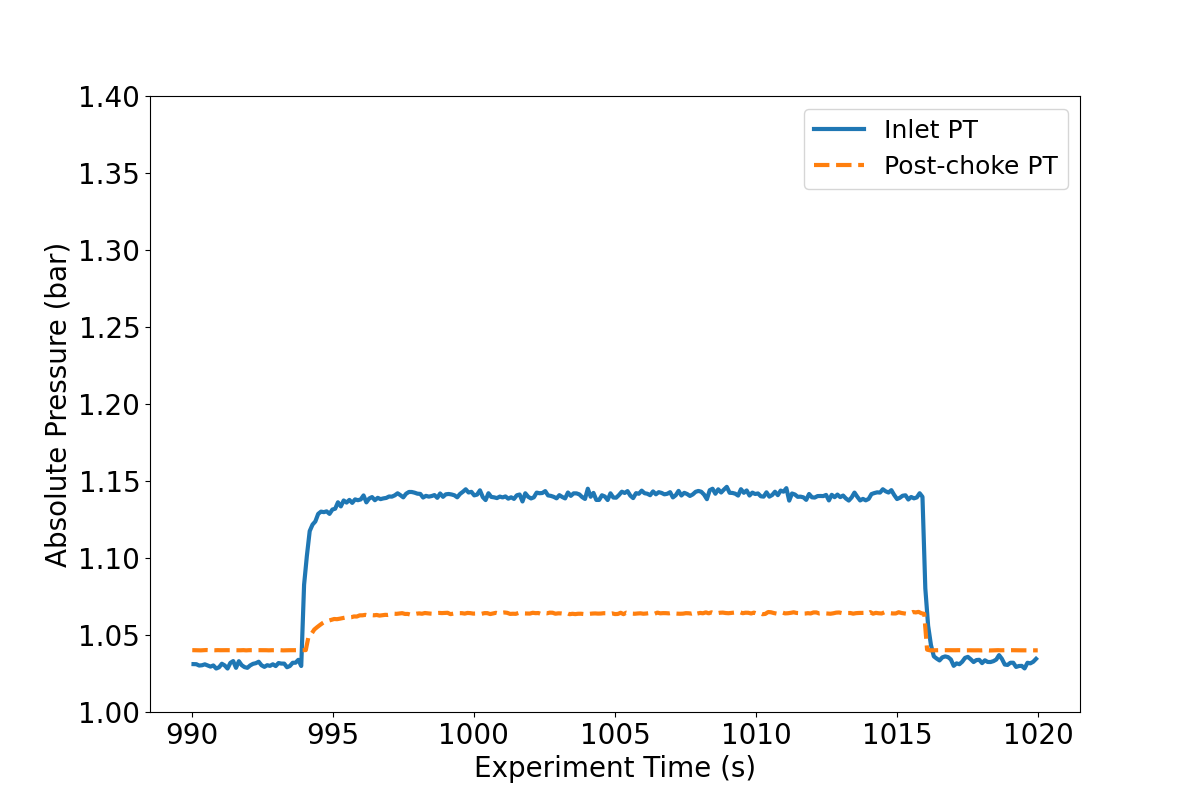
\includegraphics[width=\textwidth]{../report_assets/3_bar_static_new_reg.png}
        \caption*{(a) Testing with New Regulator}\label{fig:static-pressure-drop-new-reg}
    \end{minipage}    
    \hfill
    \begin{minipage}{0.45\textwidth}
        \centering
        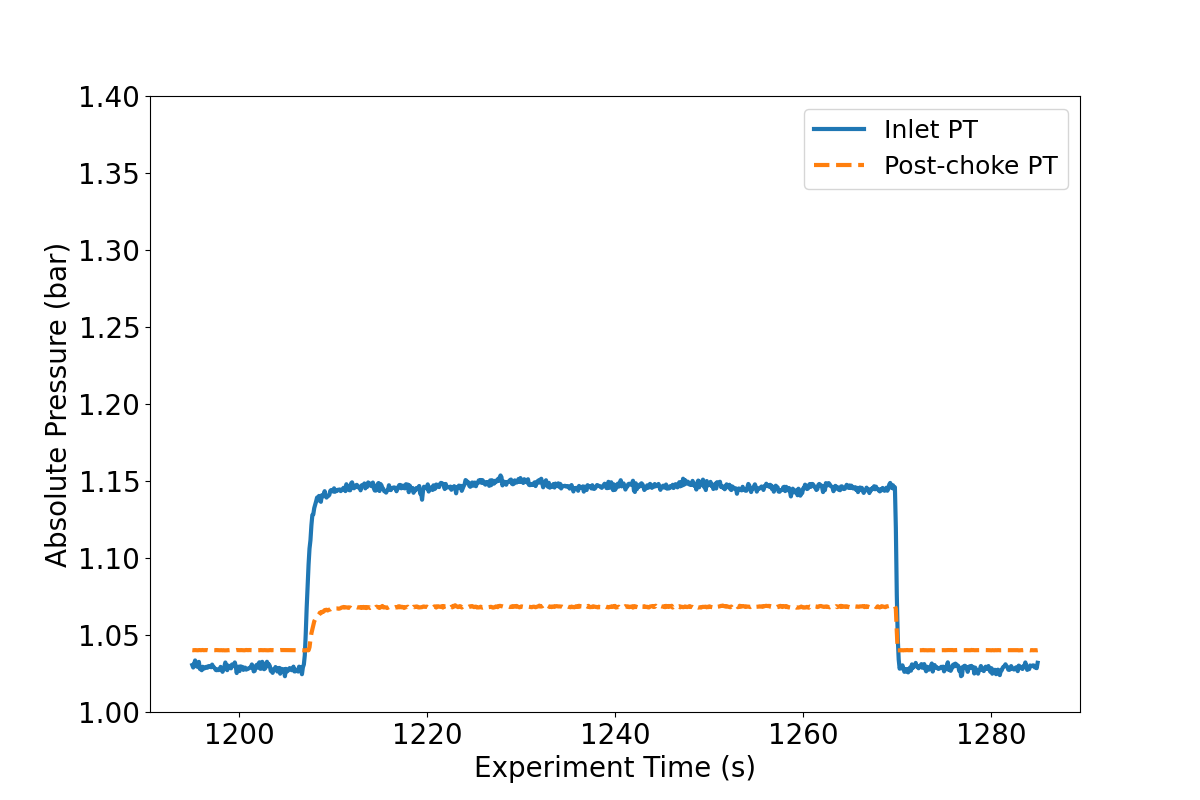
\includegraphics[width=\textwidth]{../report_assets/3_bar_static_no_solenoid.png}
        \caption*{(b) Testing with New Regulator and No Solenoid Valve}\label{fig:static-pressure-drop-no-solenoid}
    \end{minipage}    
    \caption{Follow-up 4 bar Tests with Different Configurations}\label{fig:follow-up-stat-test}
\end{figure}    


\subsection{Simulation}
From the experimental testing, two likely explanations emerged: first, the stagnation pressure supplied to the system may have been less than 4 bar due to choking upstream of the regulator; second, the static pressure readings may have been reduced by the high velocity of the flow, resulting in elevated dynamic pressure. To further investigate the system, a 2D axisymmetric steady-state simulation of the empty tank was conducted, which appeared to support both explanations. The pressure gradient observed in the simulation, shown in \autoref{fig:static-pressure-drop-fluent}, yielded results comparable to the experimental pressure transducer readings, when using a gauge pressure inlet of 1 bar.
\begin{figure}[htbp]
    \centering
    
    \begin{minipage}{0.9\textwidth}
        \centering
        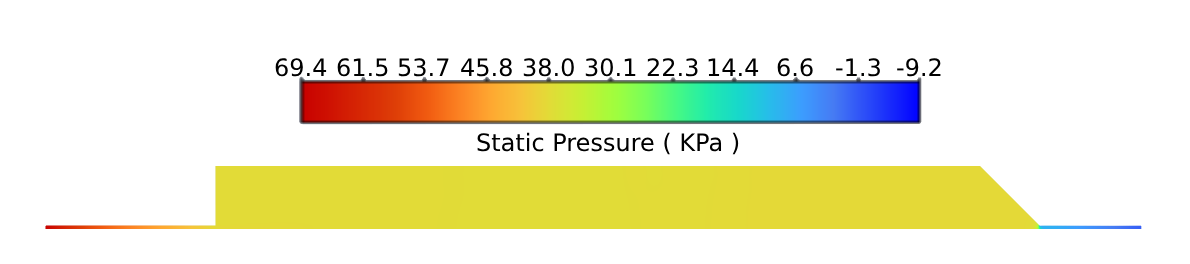
\includegraphics[width=\textwidth]{../report_assets/static_pressure_sim_results.png}
        \caption{Static Gauge Pressure of Empty Tank Simulation}\label{fig:static-pressure-drop-fluent}
    \end{minipage}    
    
\end{figure}    
The simulated pressure values at the measurement locations were 1.46 bar upstream of the tank and 1.06 bar downstream. While these are close to the experimental data, the outlet pressure was notably lower, indicating that the simulation does not fully account for the observed behaviour.

The velocity distribution from the same simulation is shown in \autoref{fig:velocity-magnitude-fluent}.
\begin{figure}[htbp]
    \centering
    
    \begin{minipage}{0.9\textwidth}
        \centering
        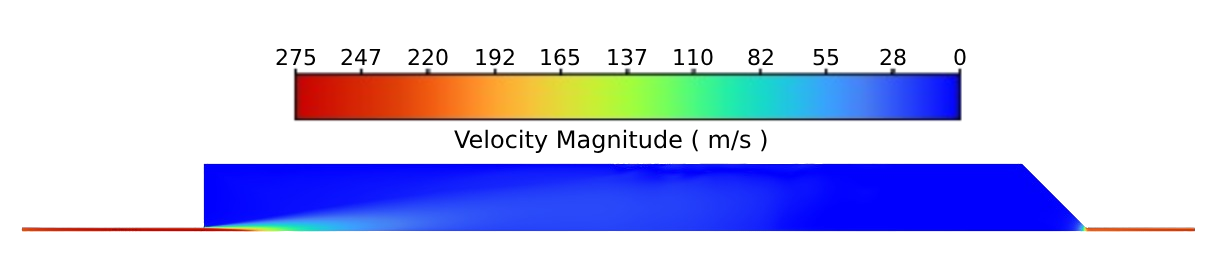
\includegraphics[width=\textwidth]{../report_assets/pressure_characterisation_vel.png}
        \caption{Velocity Magnitude of Empty Tank Simulation}\label{fig:velocity-magnitude-fluent}
    \end{minipage}    
    
\end{figure}    
Within just 0.1 m of pipe, the flow was found to accelerate to 275mm/s. This supports the hypothesis that a significant portion of the stagnation pressure is converted into dynamic pressure within the piping, which would explain the low static pressure readings observed experimentally.

\subsection{Stagnation Pressure Values}
Based on experimental testing, it was concluded that the observed behaviour was not the result of human error in setting up the system. Therefore, the hypothesised explanation is further supported by the numerical simulation, particularly with regard to the theorised high velocity in the pipes. As a result, to estimate the actual stagnation pressure at the inlet, isentropic relations were applied. Assuming the flow velocity reached Mach 1, the ratio of static to stagnation pressure is given by:
\[
\frac{p}{p_o} = 0.52828178.
\]
This relation was used to calculate the upstream stagnation pressures seen in \autoref{tab:static-stag-pressures} below.

% \begin{table}[htbp]
%     \centering
    
%     \begin{tabular}{p{0.3\textwidth} p{0.3\textwidth} p{0.3\textwidth}}
%         \hline
%         Pressure Regulator Setting (bar) & Static Pressure at Inlet (bar) &  Stagnation Pressure (bar) \\
%         \hline
%         4 & 1.405 & 2.66 \\
%         5 & 1.625 & 3.08 \\
%         6 & 1.852 & 3.51 \\
%         \hline
%     \end{tabular}    
%     \caption{Summary of static and stagnation pressures for different tests.}\label{tab:static-stag-pressures}
% \end{table}    
\begin{table}[htbp]
    \centering
    \begin{tabular}{l c c c}
        \hline
        & Test 1 & Test 2 & Test 3 \\
        \hline
        Pressure Regulator Setting (bar) & 4.00 & 5.00 & 6.00 \\
        Static Pressure at Inlet (bar) & 1.405 & 1.625 & 1.852 \\
        Stagnation Pressure (bar) & 2.66 & 3.08 & 3.51 \\
        \hline
    \end{tabular}
    \caption{Summary of Estimated Stagnation Pressures for Each Test}\label{tab:static-stag-pressures}
\end{table}


\newpage

\section{Mass Flow Rate Experiment}
\subsection{Results from an Inlet Pressure of 4 bar}
\vfill

\begin{figure}[htbp]
    \centering

    \begin{minipage}{0.32\textwidth}
        \centering
        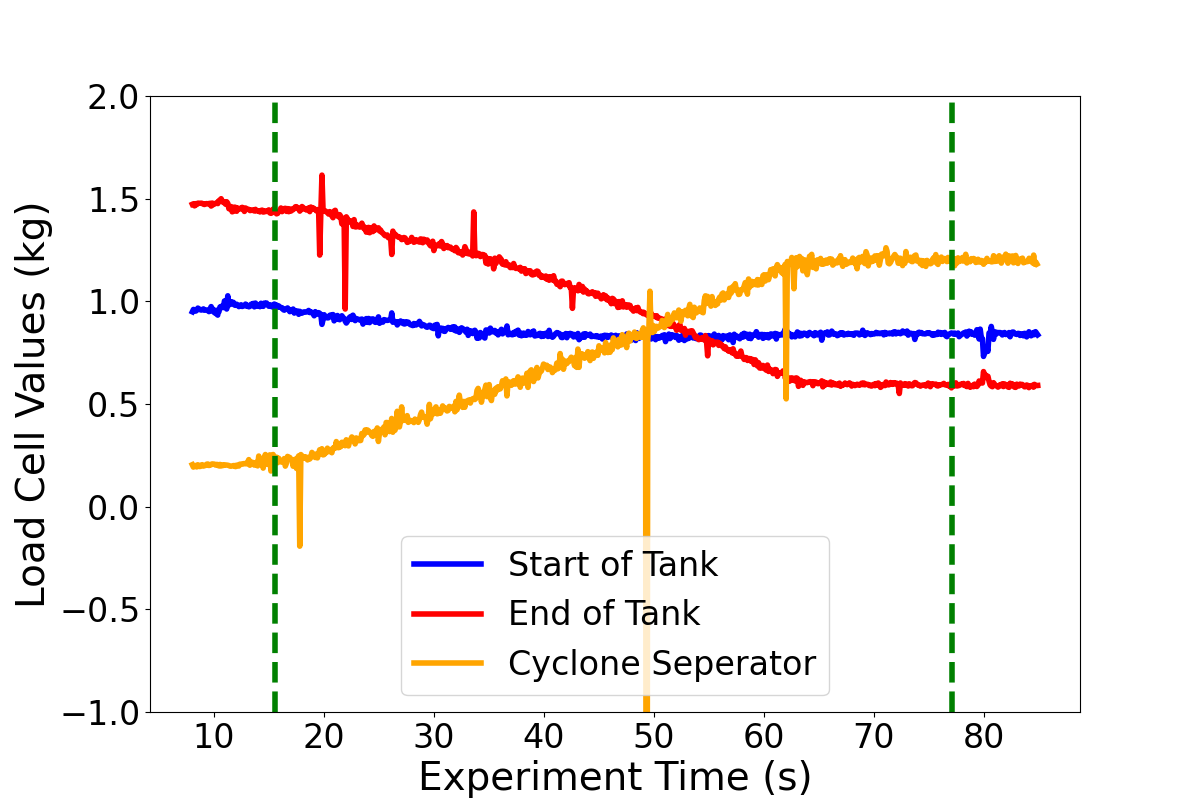
\includegraphics[width=\textwidth]{../report_assets/41_raw_mass.png}
        \caption*{(a) Raw Load Cell Readings}
    \end{minipage}
    \hfill
    \begin{minipage}{0.32\textwidth}
        \centering
        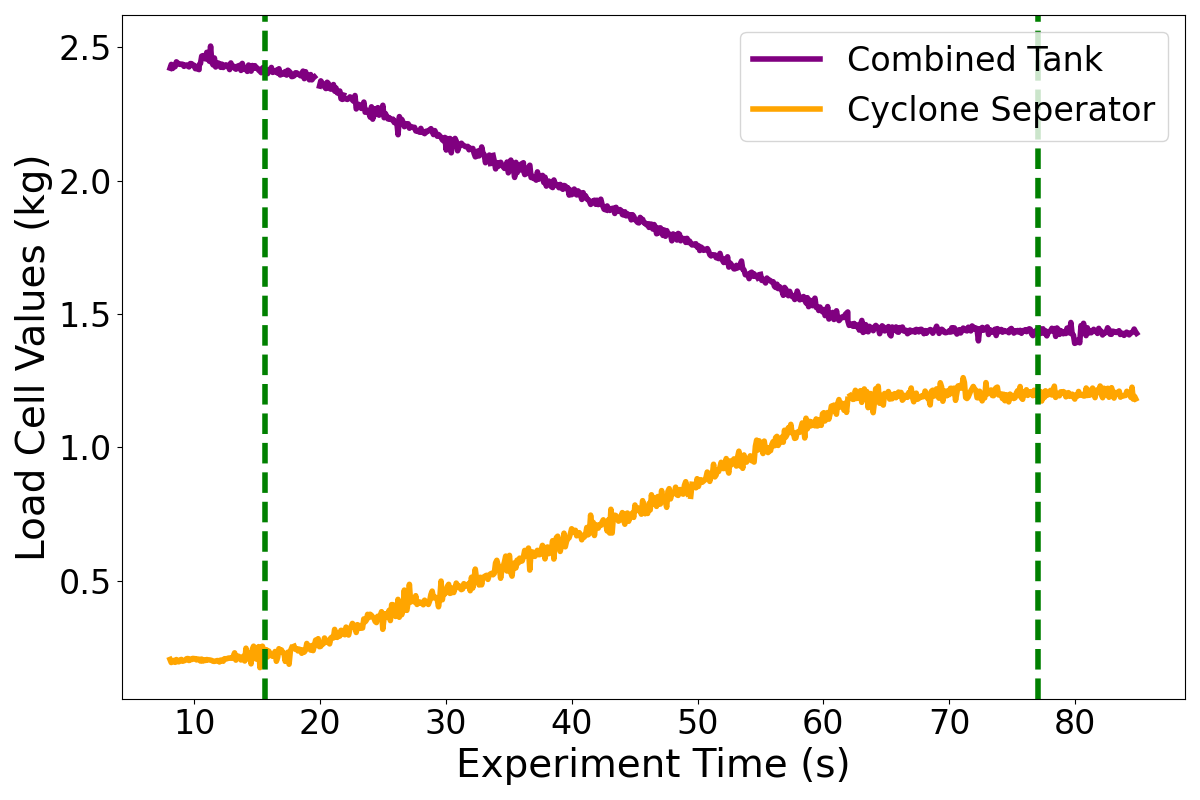
\includegraphics[width=\textwidth]{../report_assets/41_clean_mass.png}
        \caption*{(b) Cleaned Mass Change}
    \end{minipage}
    \hfill
    \begin{minipage}{0.32\textwidth}
        \centering
        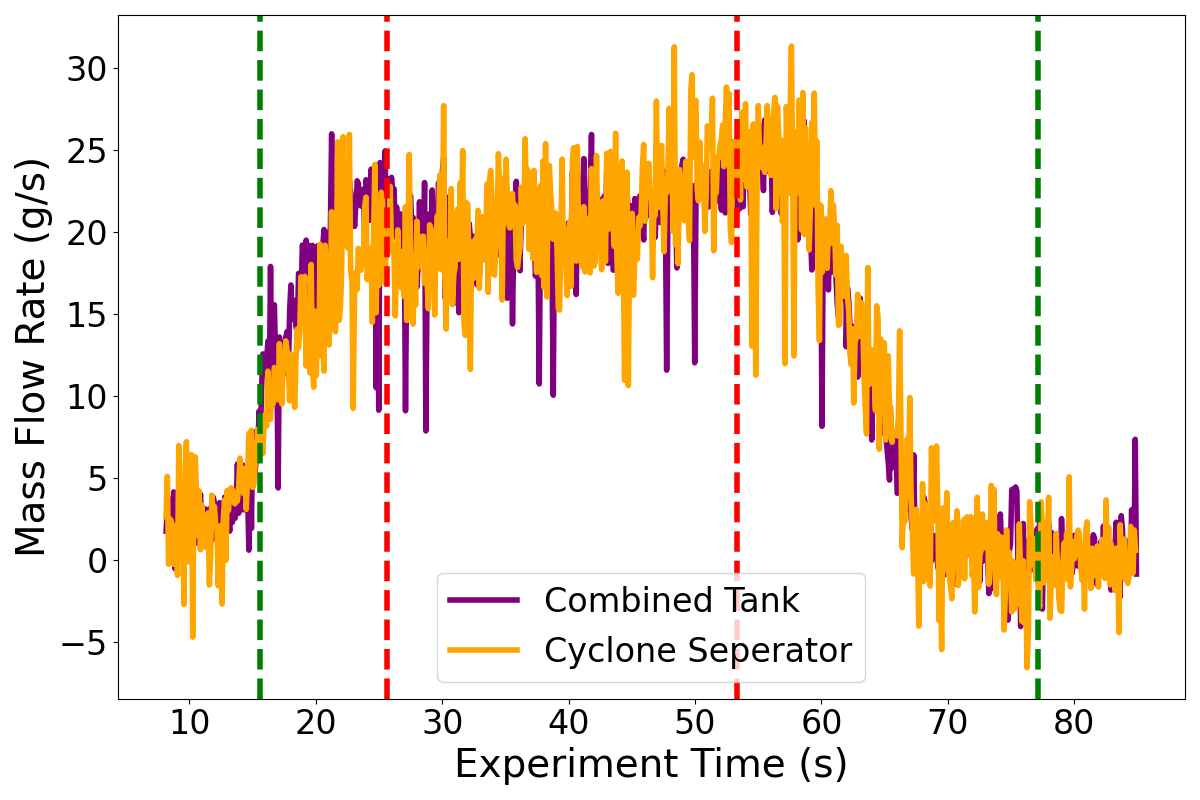
\includegraphics[width=\textwidth]{../report_assets/41_clean_flow_100.png}
        \caption*{(c) Mass Flow Rate}
    \end{minipage}
    \caption{1st Test Using a 4 bar Inlet Pressure}

\end{figure}\label{fig:41}
\vfill
\begin{figure}[htbp]
    \centering

    \begin{minipage}{0.32\textwidth}
        \centering
        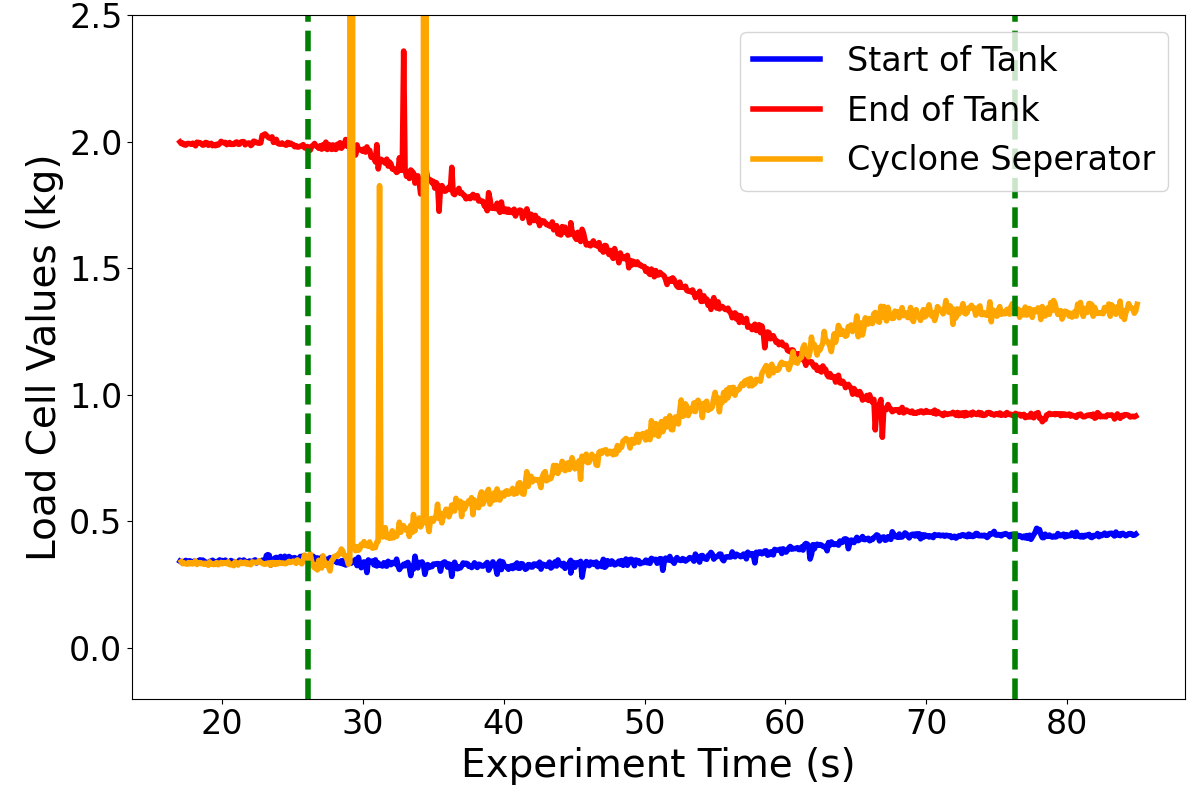
\includegraphics[width=\textwidth]{../report_assets/42_raw_mass.png}
        \caption*{(a) Raw Load Cell Readings}
    \end{minipage}
    \hfill
    \begin{minipage}{0.32\textwidth}
        \centering
        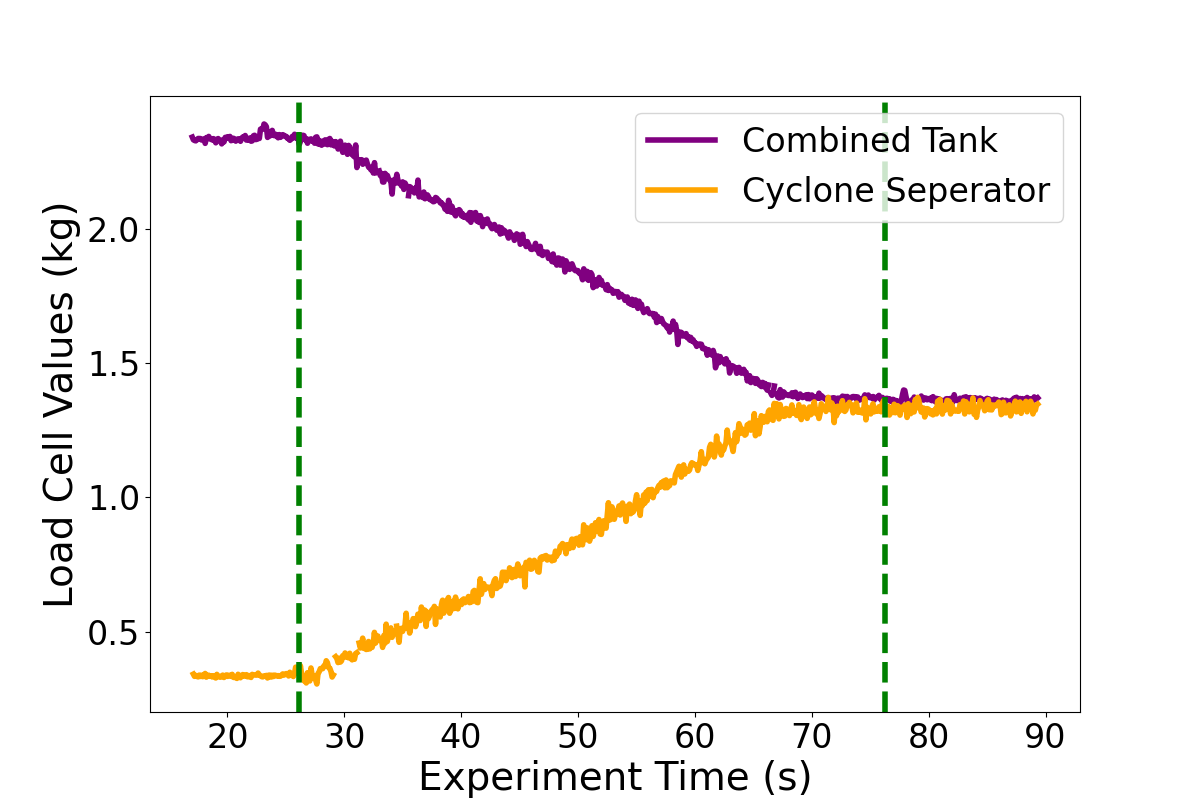
\includegraphics[width=\textwidth]{../report_assets/42_clean_mass.png}
        \caption*{(b) Cleaned Mass Change}
    \end{minipage}
    \hfill
    \begin{minipage}{0.32\textwidth}
        \centering
        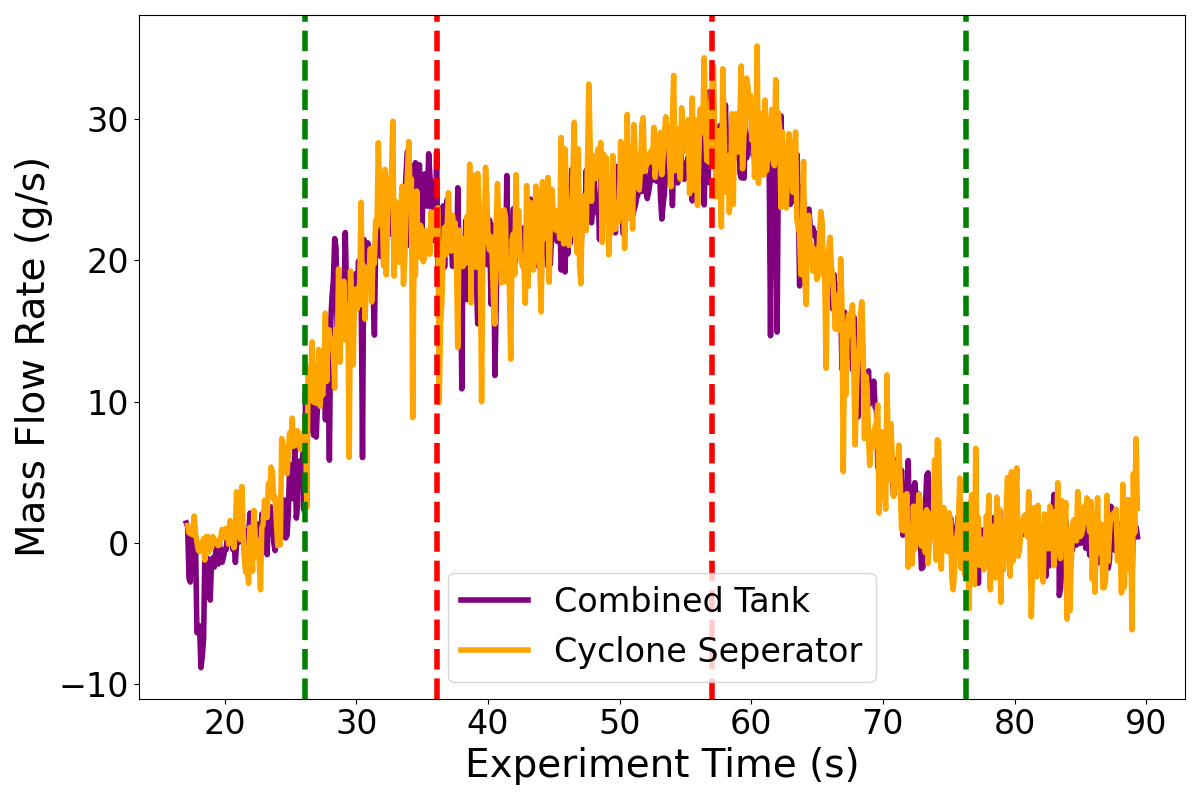
\includegraphics[width=\textwidth]{../report_assets/42_clean_flow_100.png}
        \caption*{(c) Mass Flow Rate}
    \end{minipage}
    \caption{2nd Test Using a 4 bar Inlet Pressure}
    
\end{figure}\label{fig:42}
\vfill
\begin{figure}[htbp]
    \centering

    \begin{minipage}{0.32\textwidth}
        \centering
        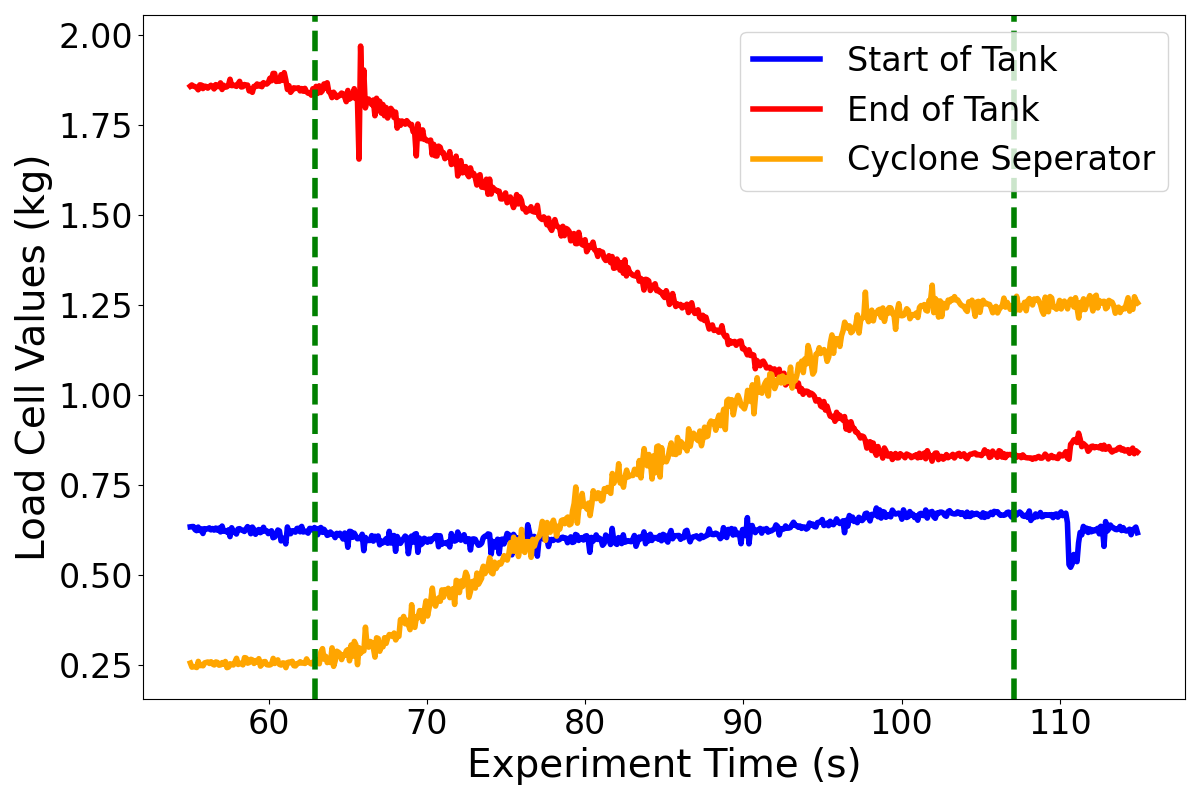
\includegraphics[width=\textwidth]{../report_assets/43_raw_mass.png}
        \caption*{(a) Raw Load Cell Readings}
    \end{minipage}
    \hfill
    \begin{minipage}{0.32\textwidth}
        \centering
        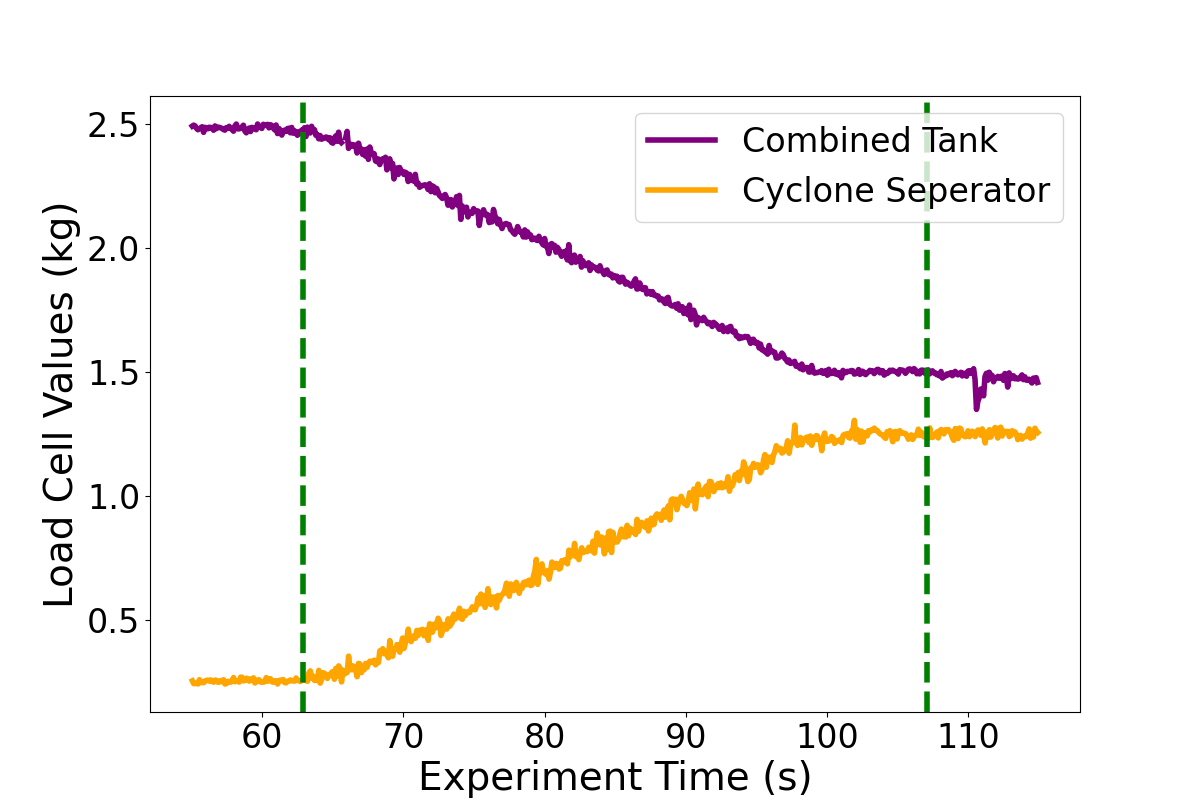
\includegraphics[width=\textwidth]{../report_assets/43_clean_mass.png}
        \caption*{(b) Cleaned Mass Change}
    \end{minipage}
    \hfill
    \begin{minipage}{0.32\textwidth}
        \centering
        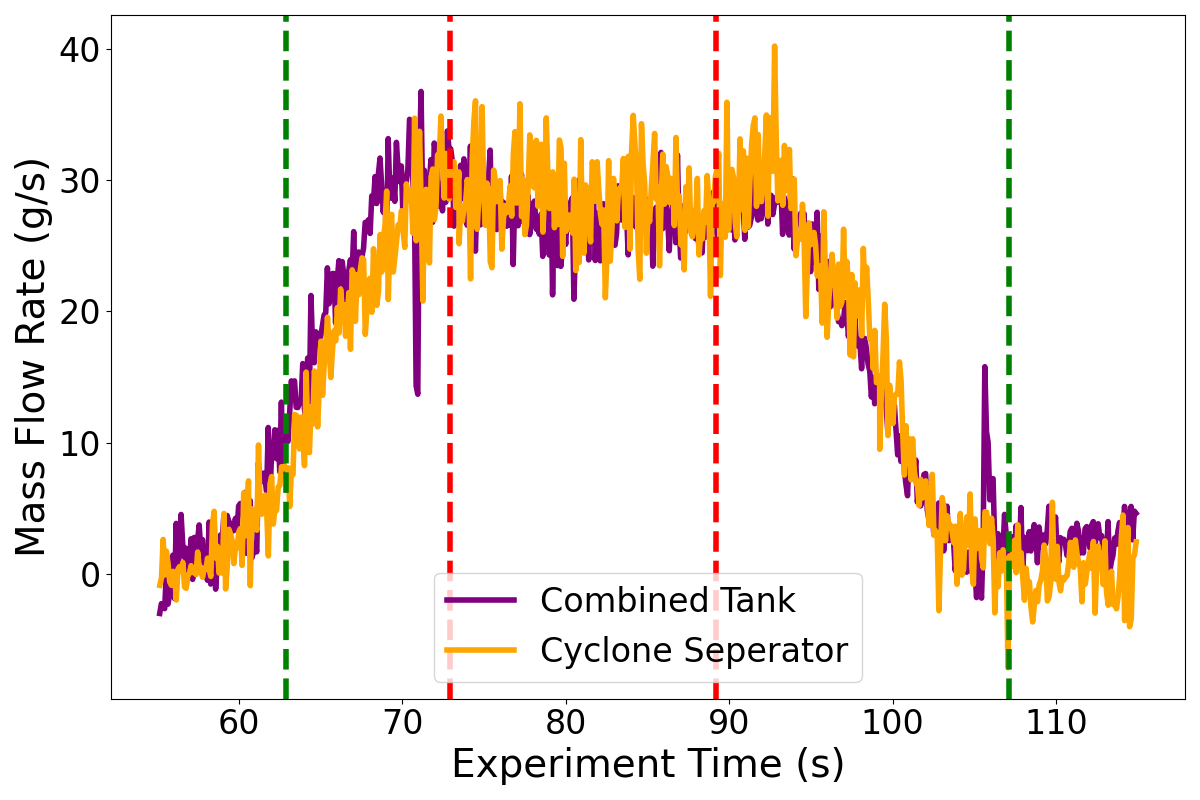
\includegraphics[width=\textwidth]{../report_assets/43_clean_flow_100.png}
        \caption*{(c) Mass Flow Rate}
    \end{minipage}
    \caption{3rd Test Using a 4 bar Inlet Pressure}
    
\end{figure}\label{fig:43}
\vfill

\newpage

\subsection{Results from an Inlet Pressure of 5 bar}
\vfill
\begin{figure}[htbp]
    \centering

    \begin{minipage}{0.32\textwidth}
        \centering
        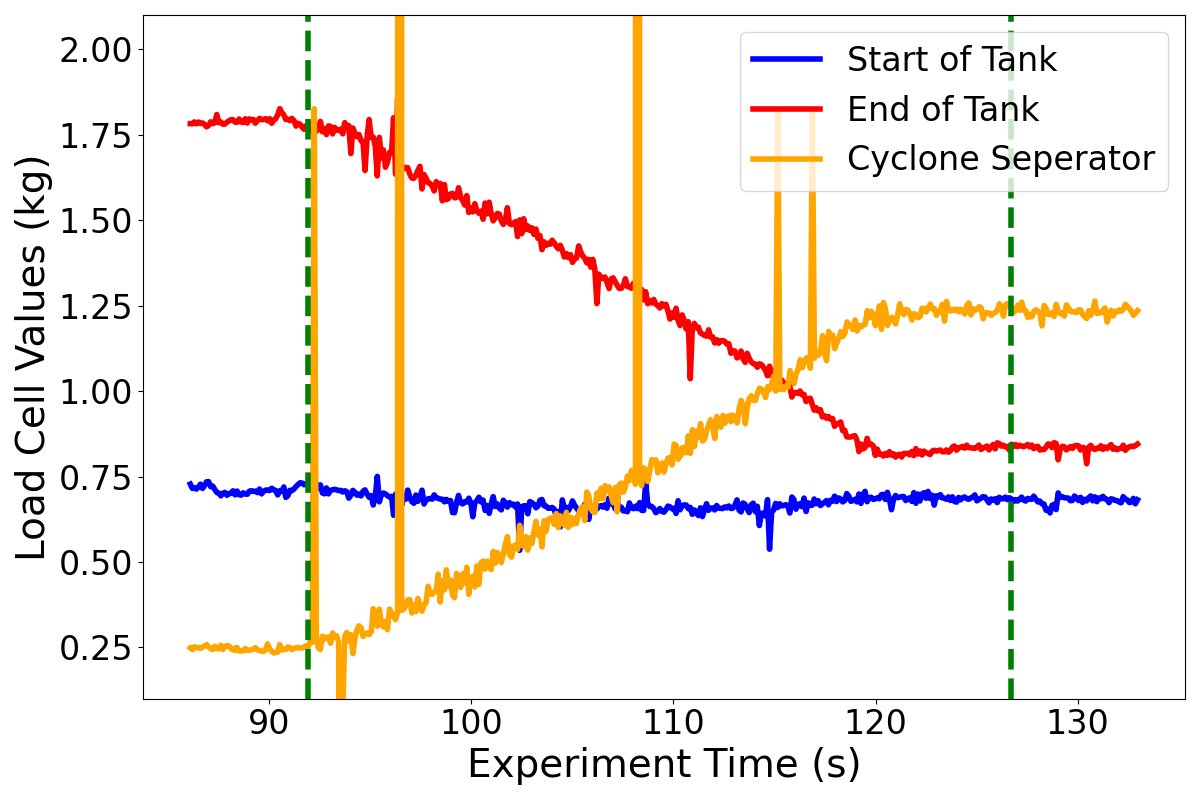
\includegraphics[width=\textwidth]{../report_assets/51_raw_mass.png}
        \caption*{(a) Raw Load Cell Readings}
    \end{minipage}
    \hfill
    \begin{minipage}{0.32\textwidth}
        \centering
        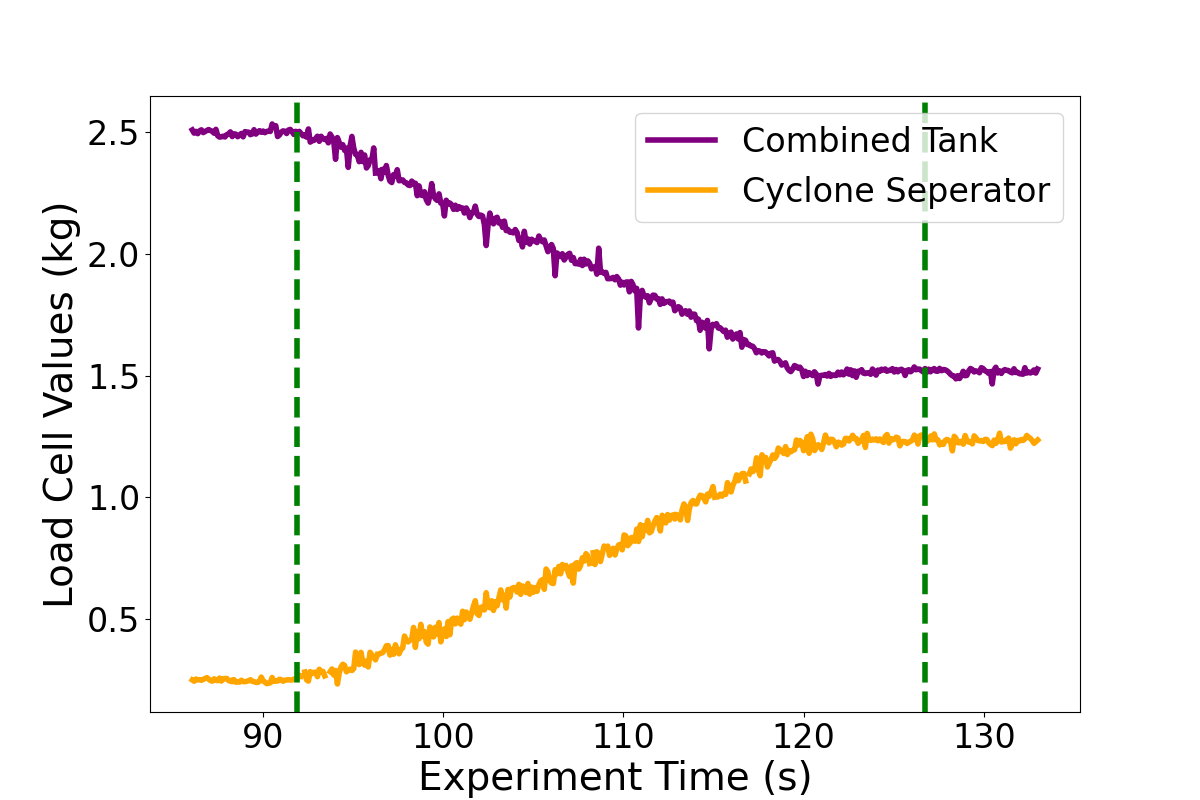
\includegraphics[width=\textwidth]{../report_assets/51_clean_mass.png}
        \caption*{(b) Cleaned Mass Change}
    \end{minipage}
    \hfill
    \begin{minipage}{0.32\textwidth}
        \centering
        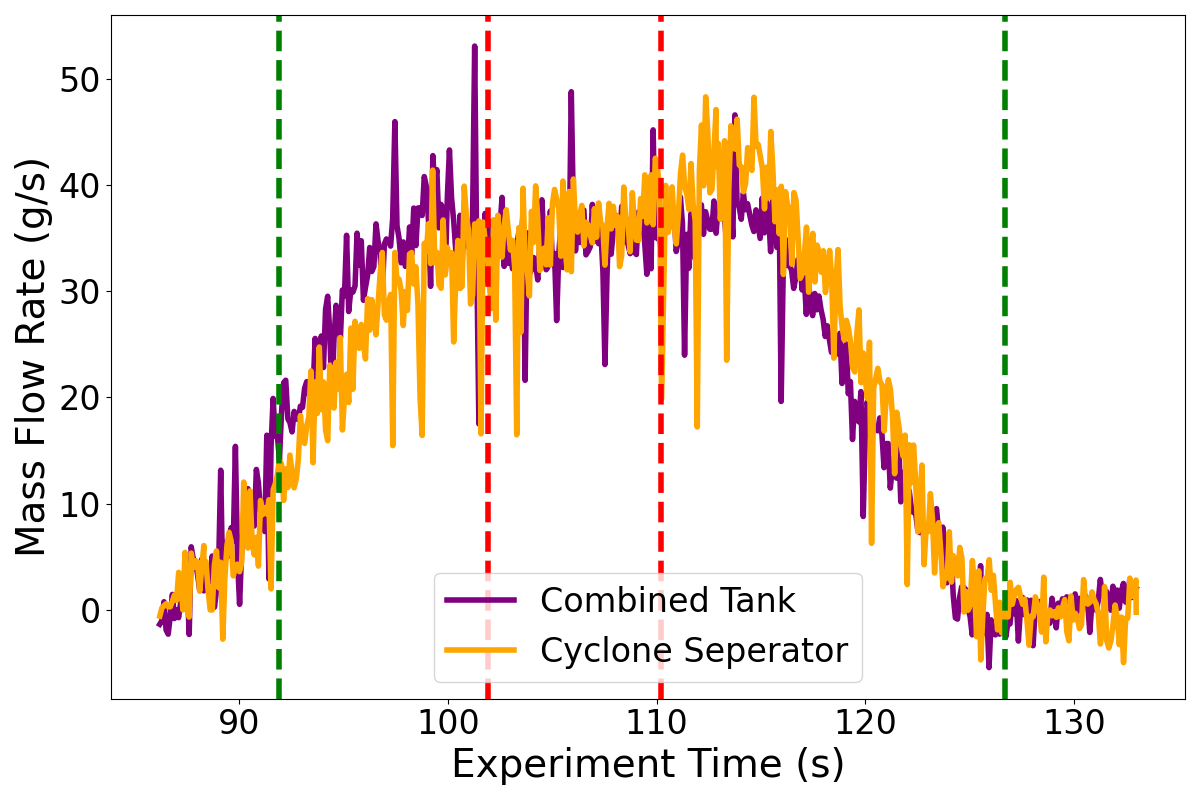
\includegraphics[width=\textwidth]{../report_assets/51_clean_flow_100.png}
        \caption*{(c) Mass Flow Rate}
    \end{minipage}
    \caption{1st Test Using a 5 bar Inlet Pressure}
    
\end{figure}\label{fig:51}
\vfill

\begin{figure}[htbp]
    \centering

    \begin{minipage}{0.32\textwidth}
        \centering
        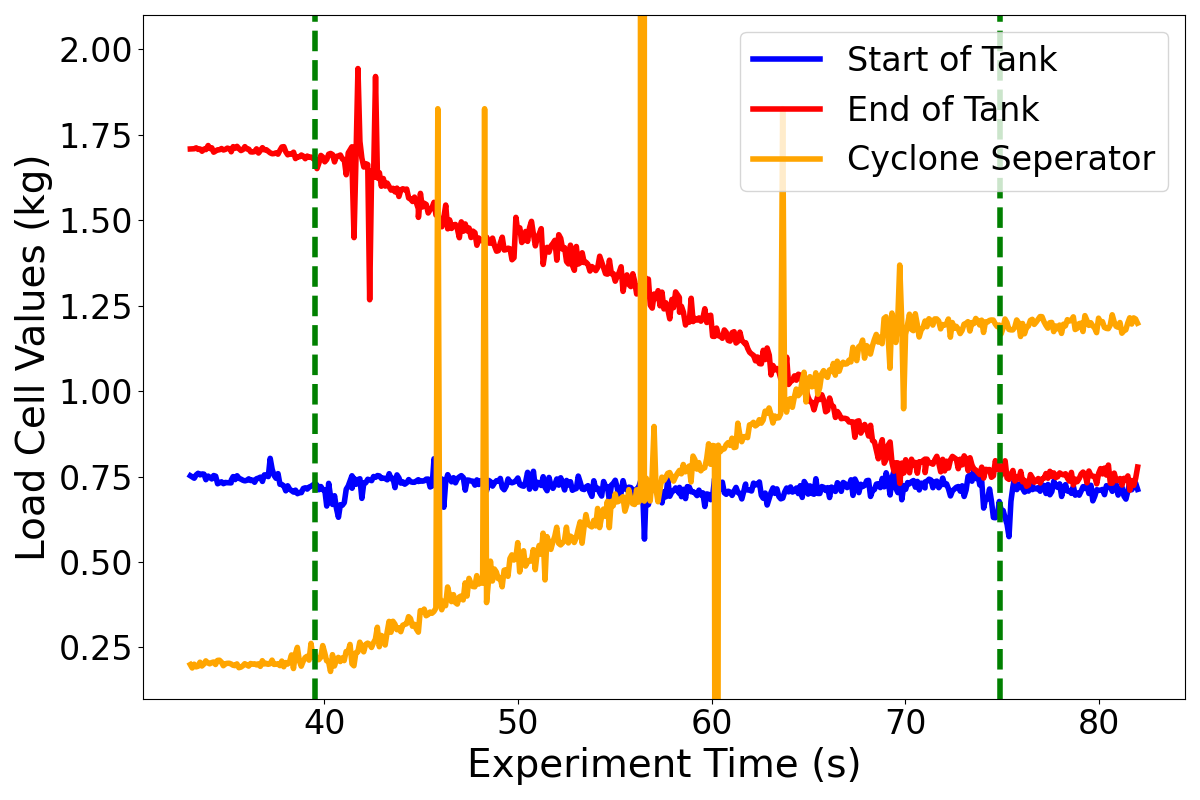
\includegraphics[width=\textwidth]{../report_assets/52_raw_mass.png}
        \caption*{(a) Raw Load Cell Readings}
    \end{minipage}
    \hfill
    \begin{minipage}{0.32\textwidth}
        \centering
        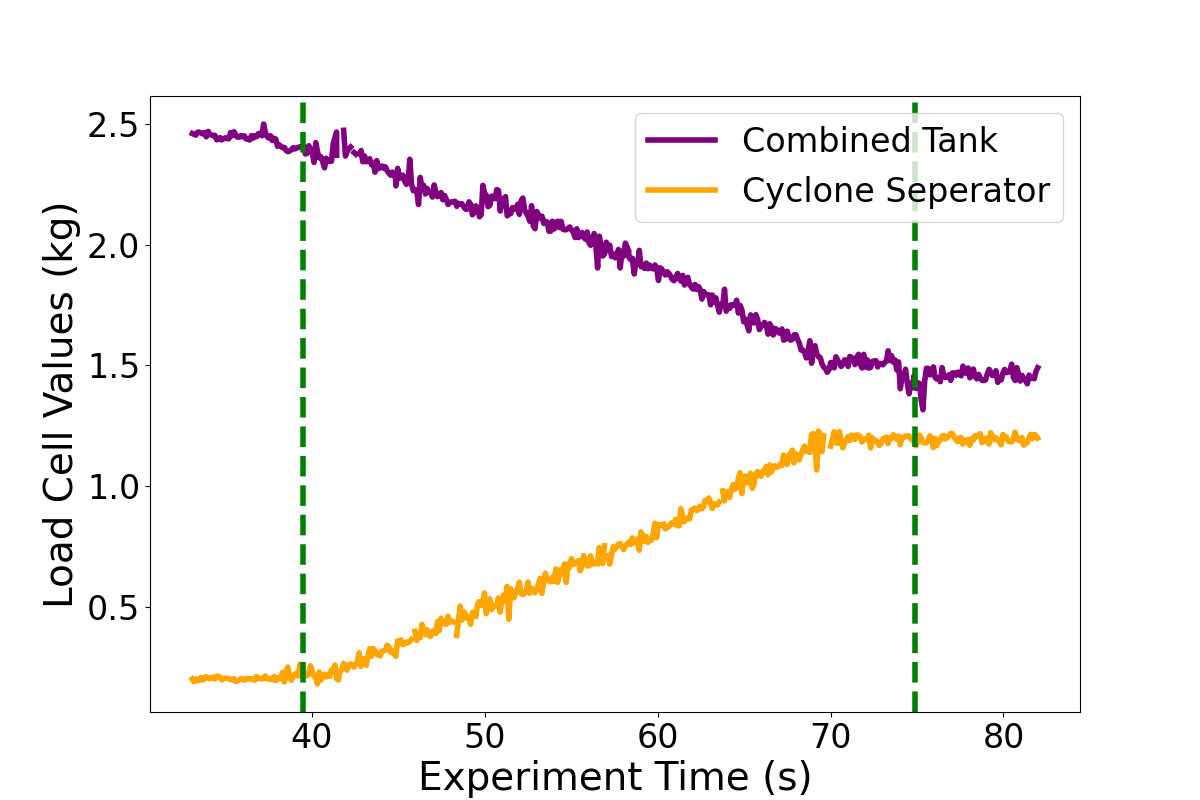
\includegraphics[width=\textwidth]{../report_assets/52_clean_mass.png}
        \caption*{(b) Cleaned Mass Change}
    \end{minipage}
    \hfill
    \begin{minipage}{0.32\textwidth}
        \centering
        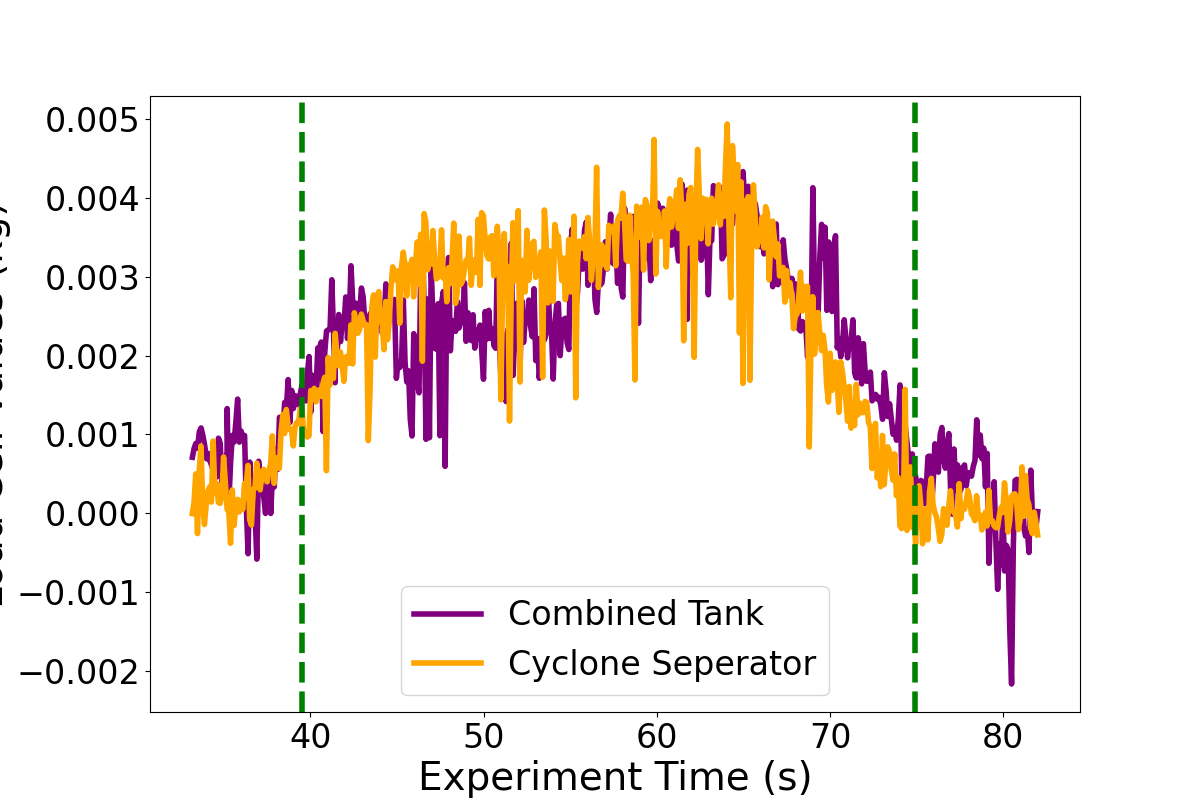
\includegraphics[width=\textwidth]{../report_assets/52_clean_flow_100.png}
        \caption*{(c) Mass Flow Rate}
    \end{minipage}
    \caption{2nd Test Using a 5 bar Inlet Pressure}
    
\end{figure}\label{fig:52}
\vfill

\begin{figure}[htbp]
    \centering

    \begin{minipage}{0.32\textwidth}
        \centering
        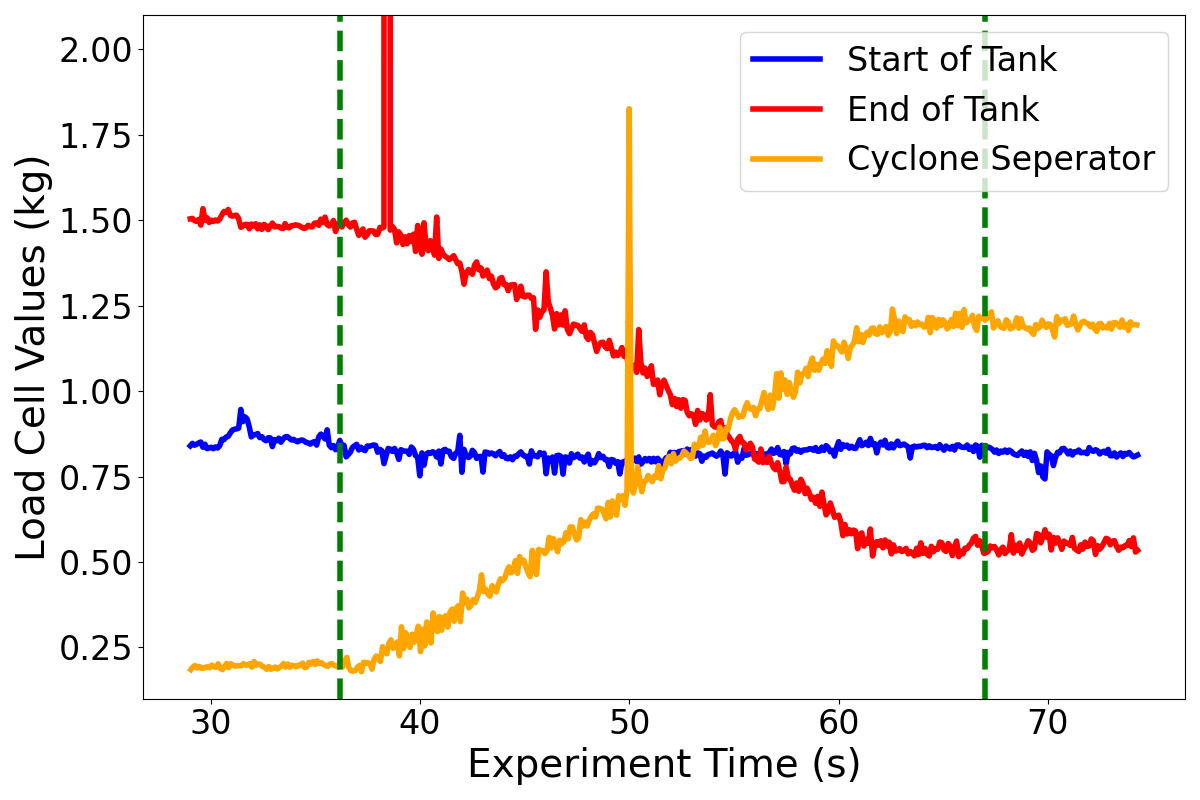
\includegraphics[width=\textwidth]{../report_assets/53_raw_mass.png}
        \caption*{(a) Raw Load Cell Readings}
    \end{minipage}
    \hfill
    \begin{minipage}{0.32\textwidth}
        \centering
        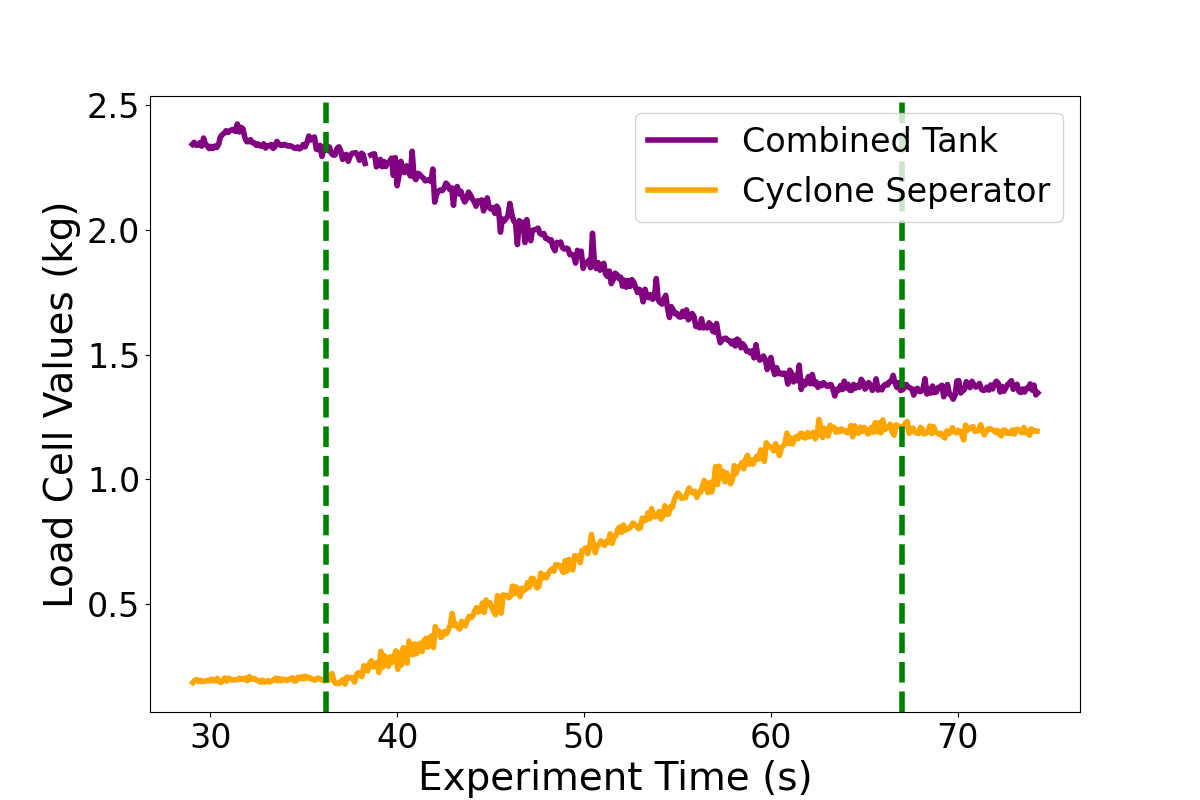
\includegraphics[width=\textwidth]{../report_assets/53_clean_mass.png}
        \caption*{(b) Cleaned Mass Change}
    \end{minipage}
    \hfill
    \begin{minipage}{0.32\textwidth}
        \centering
        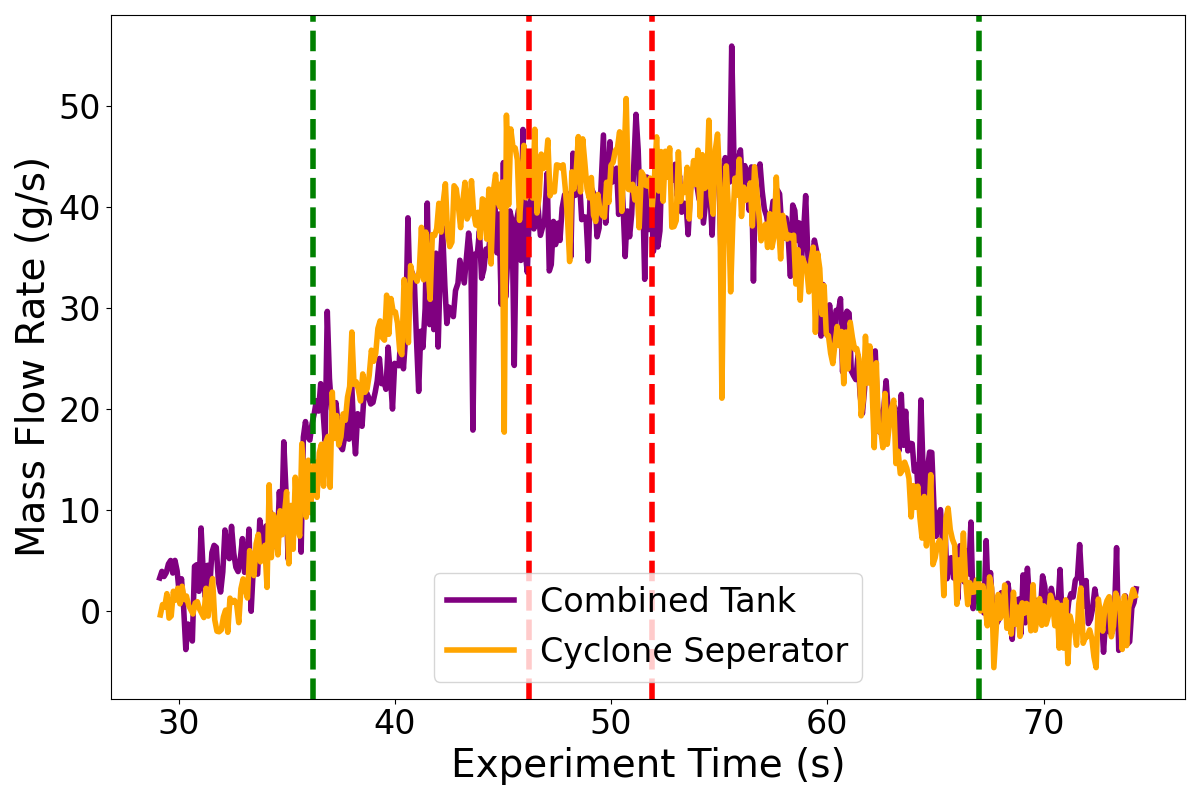
\includegraphics[width=\textwidth]{../report_assets/53_clean_flow_100.png}
        \caption*{(c) Mass Flow Rate}
    \end{minipage}
    \caption{3rd Test Using a 5 bar Inlet Pressure}
    
\end{figure}\label{fig:53}
\vfill
\newpage

\subsection{Results from an Inlet Pressure of 6 bar}
\vfill
\begin{figure}[htbp]
    \centering

    \begin{minipage}{0.32\textwidth}
        \centering
        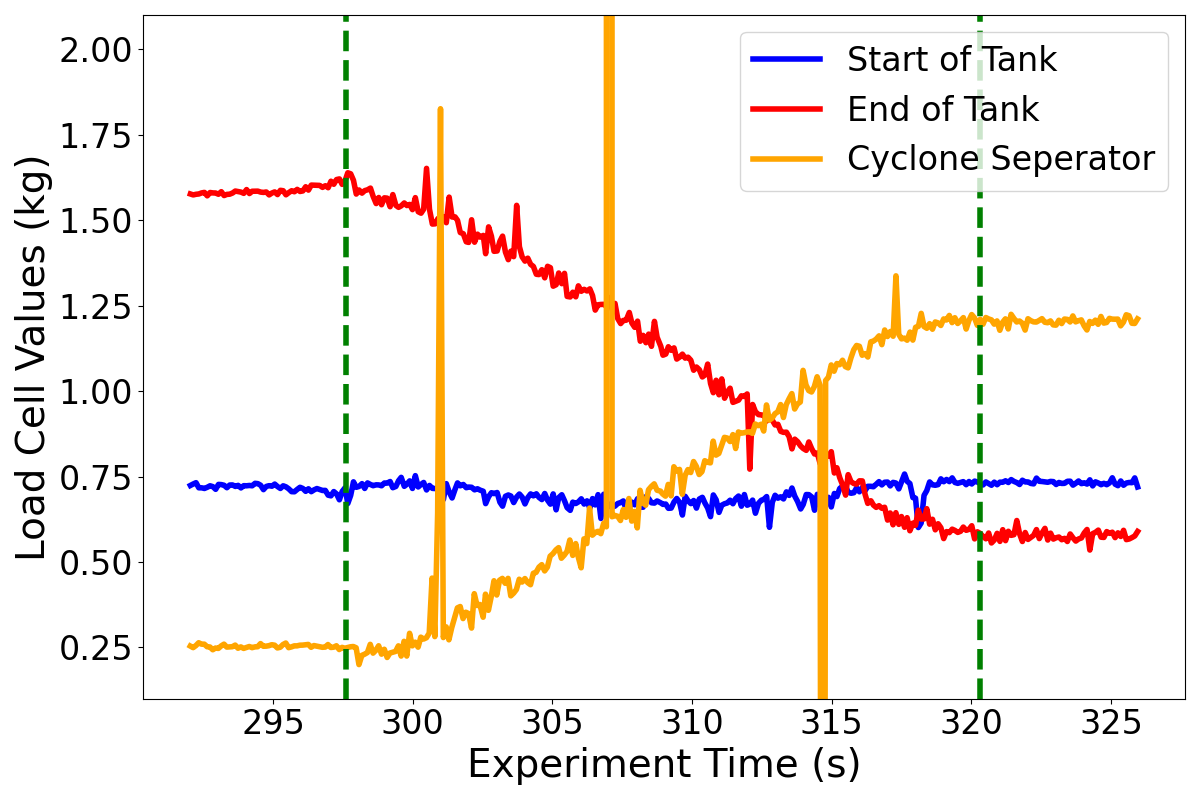
\includegraphics[width=\textwidth]{../report_assets/61_raw_mass.png}
        \caption*{(a) Raw Load Cell Readings}
    \end{minipage}
    \hfill
    \begin{minipage}{0.32\textwidth}
        \centering
        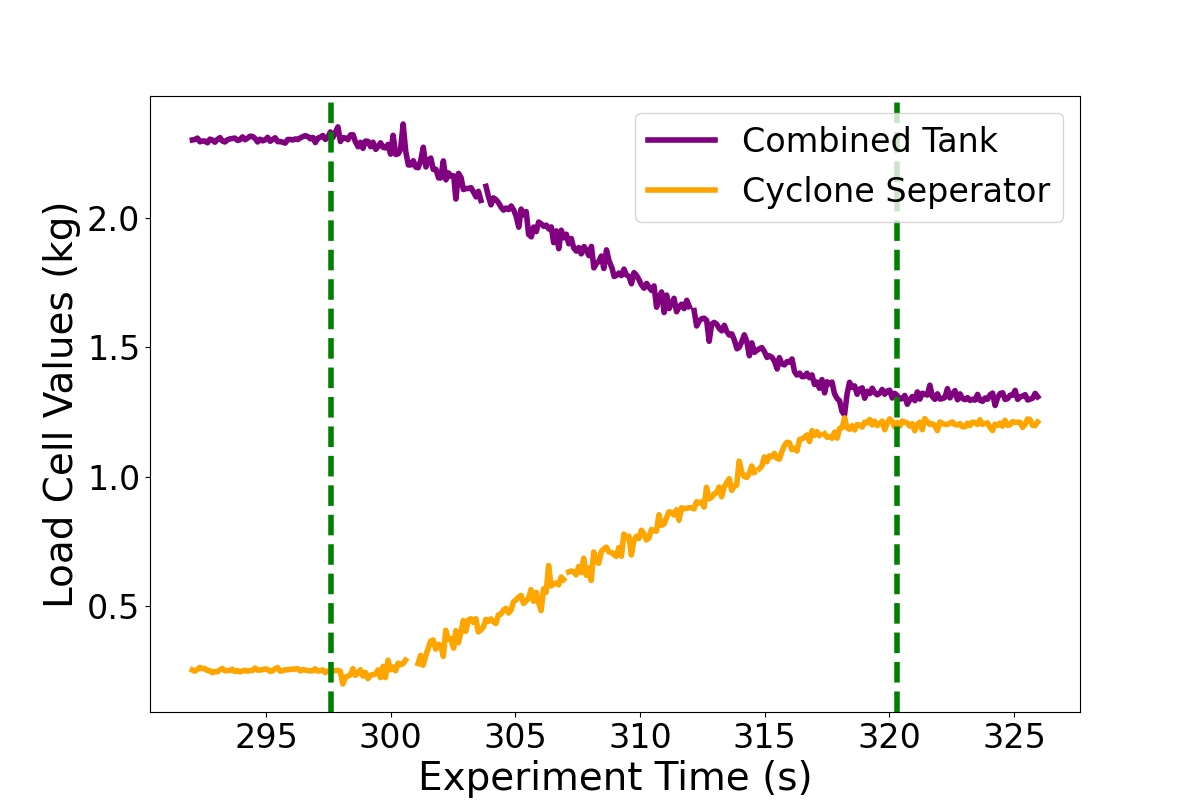
\includegraphics[width=\textwidth]{../report_assets/61_clean_mass.png}
        \caption*{(b) Cleaned Mass Change}
    \end{minipage}
    \hfill
    \begin{minipage}{0.32\textwidth}
        \centering
        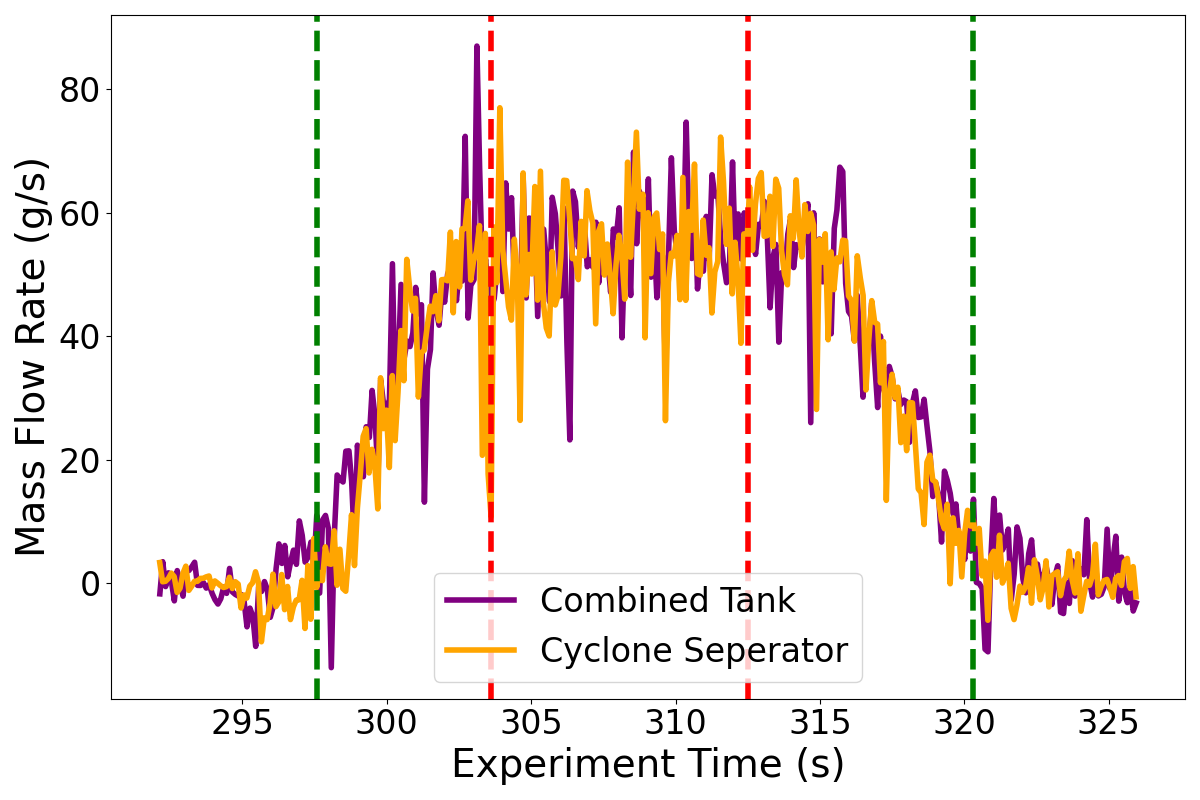
\includegraphics[width=\textwidth]{../report_assets/61_clean_flow_50.png}
        \caption*{(c) Mass Flow Rate}
    \end{minipage}
    \caption{1st Test Using a 6 bar Inlet Pressure}
    
\end{figure}\label{fig:61}

\vfill
\begin{figure}[htbp]
    \centering

    \begin{minipage}{0.32\textwidth}
        \centering
        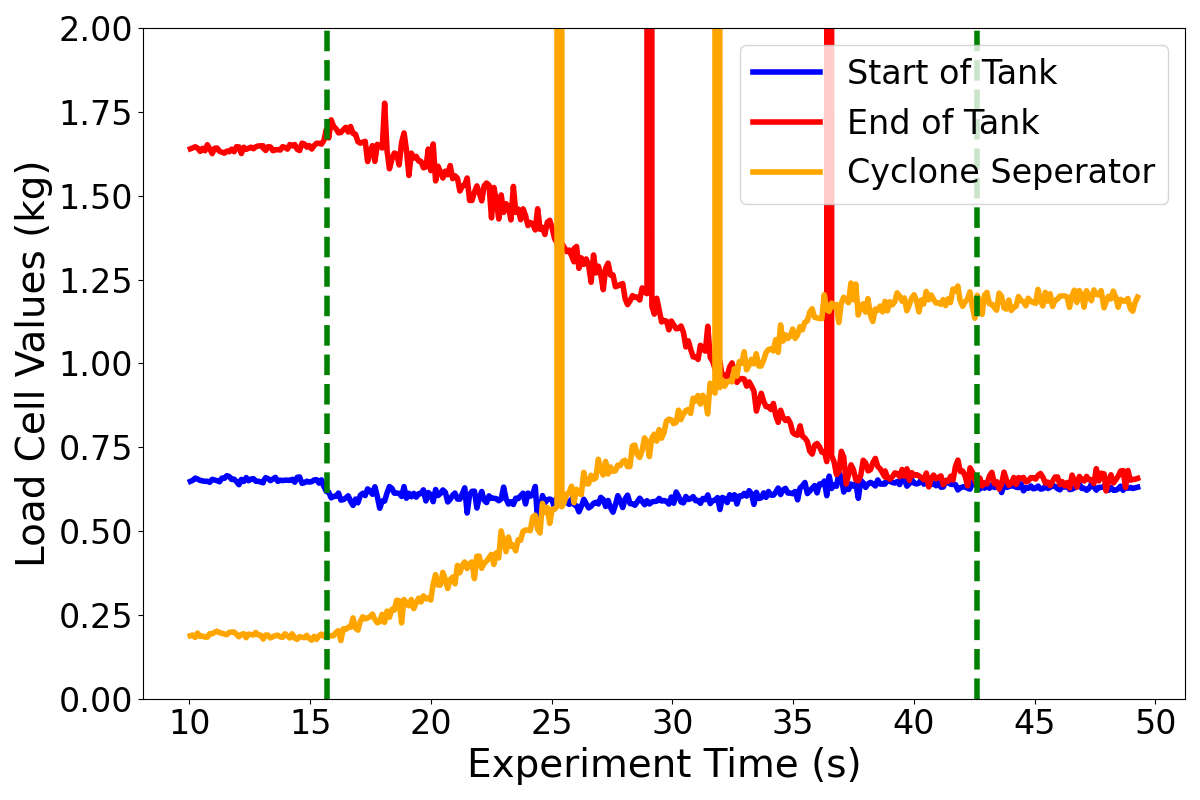
\includegraphics[width=\textwidth]{../report_assets/63_raw_mass.png}
        \caption*{(a) Raw Load Cell Readings}
    \end{minipage}
    \hfill
    \begin{minipage}{0.32\textwidth}
        \centering
        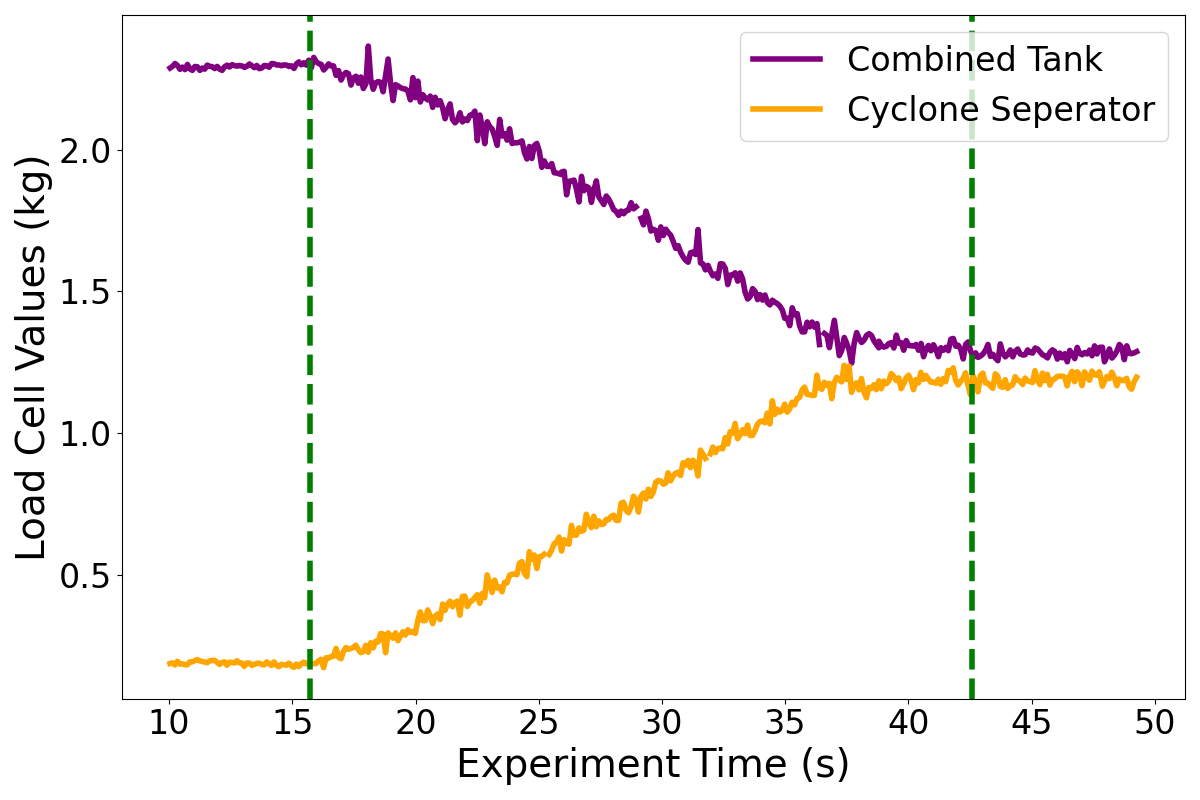
\includegraphics[width=\textwidth]{../report_assets/63_clean_mass.png}
        \caption*{(b) Cleaned Mass Change}
    \end{minipage}
    \hfill
    \begin{minipage}{0.32\textwidth}
        \centering
        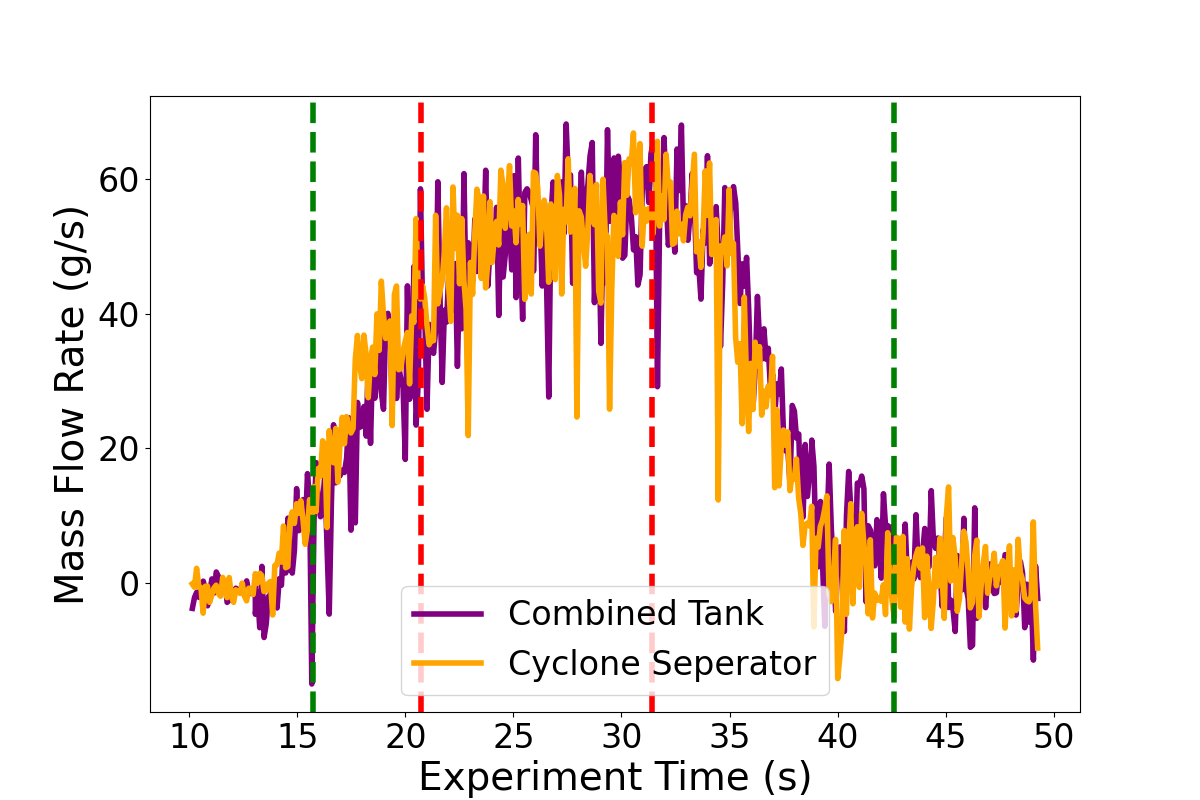
\includegraphics[width=\textwidth]{../report_assets/63_clean_flow_50.png}
        \caption*{(c) Mass Flow Rate}
    \end{minipage}
    \caption{2nd Test Using a 6 bar Inlet Pressure}
    
\end{figure}\label{fig:63}

\vfill
\begin{figure}[htbp]
    \centering

    \begin{minipage}{0.32\textwidth}
        \centering
        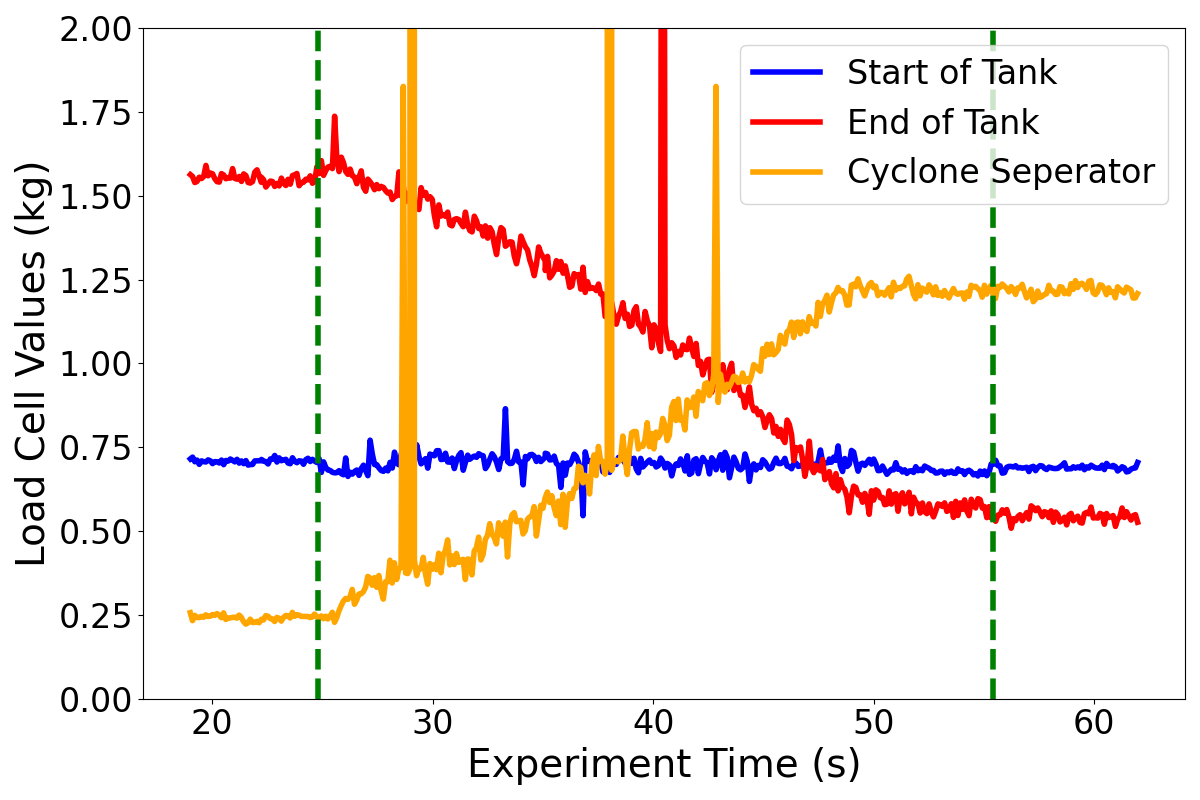
\includegraphics[width=\textwidth]{../report_assets/64_raw_mass.png}
        \caption*{(a) Raw Load Cell Readings}
    \end{minipage}
    \hfill
    \begin{minipage}{0.32\textwidth}
        \centering
        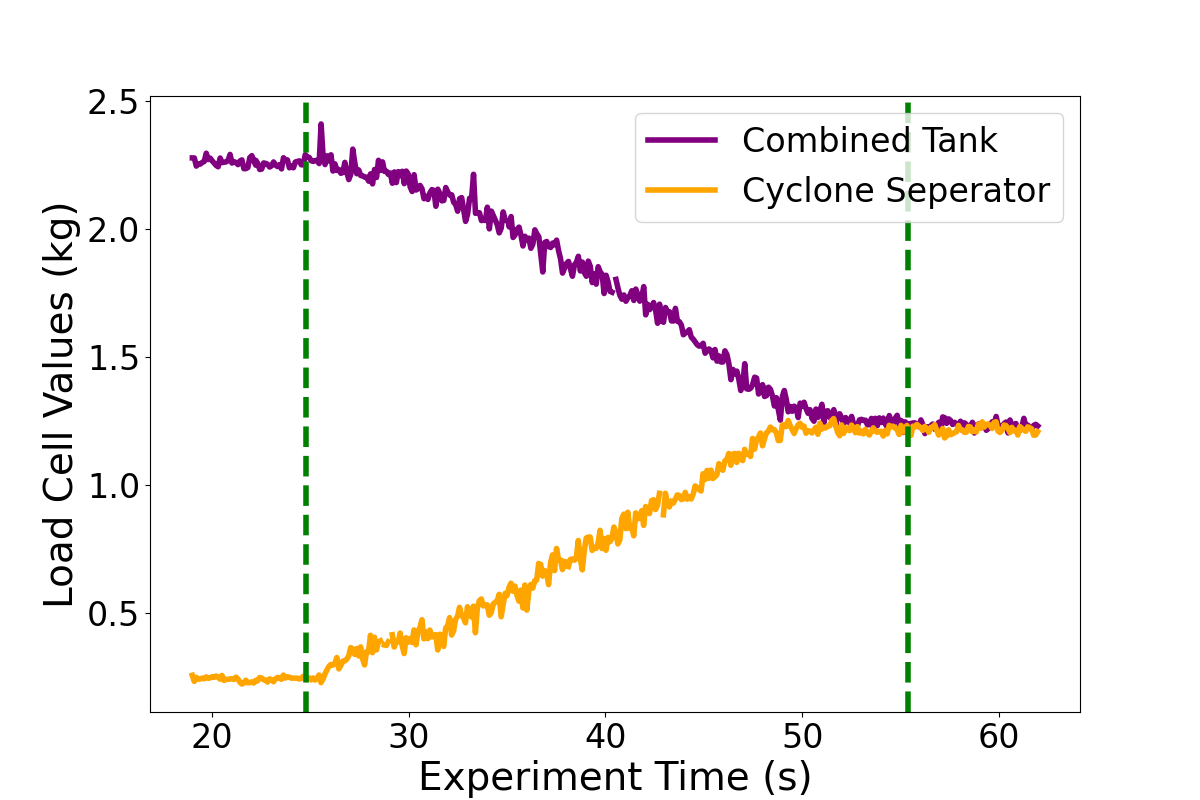
\includegraphics[width=\textwidth]{../report_assets/64_clean_mass.png}
        \caption*{(b) Cleaned Mass Change}
    \end{minipage}
    \hfill
    \begin{minipage}{0.32\textwidth}
        \centering
        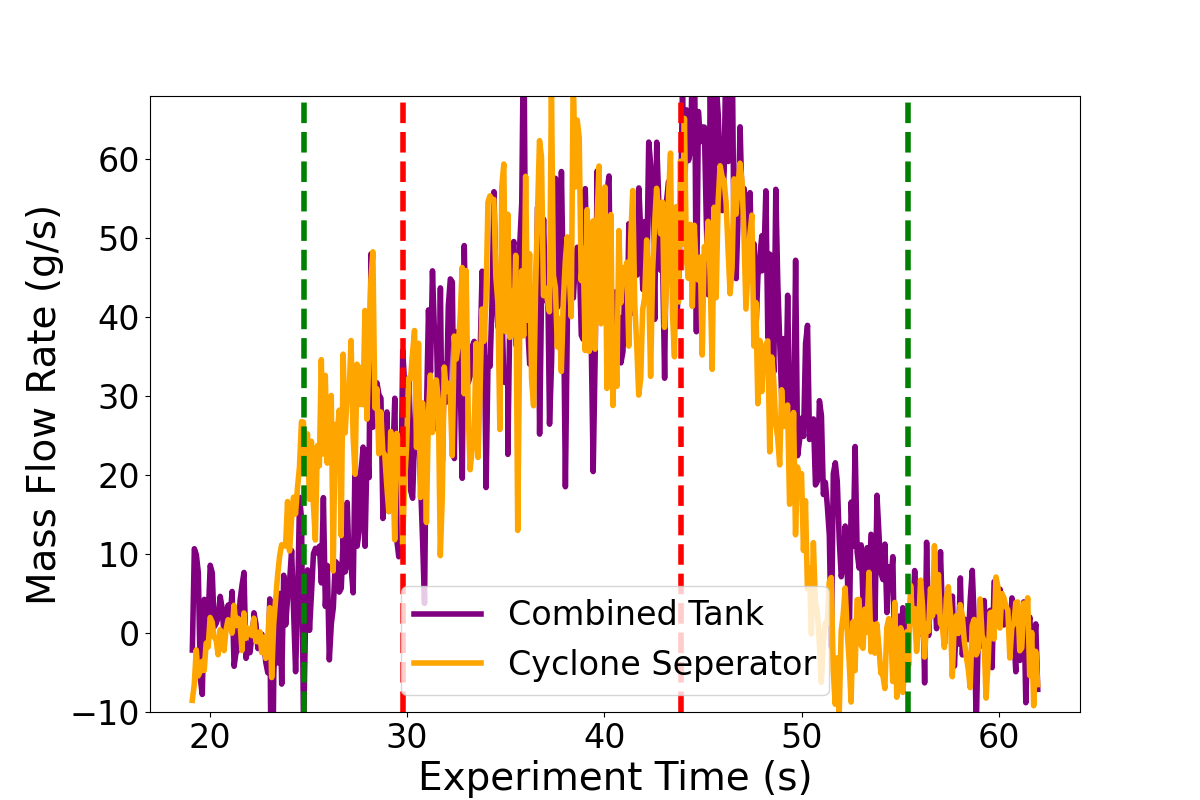
\includegraphics[width=\textwidth]{../report_assets/64_clean_flow_50.png}
        \caption*{(c) Mass Flow Rate}
    \end{minipage}
    \caption{3rd Test Using a 6 bar Inlet Pressure}
    
\end{figure}\label{fig:64}
\vfill
\newpage

\subsection{Mass Flow Rate Analysis and Discussion}
For each test, the raw load cell readings are shown in graphs (a) above. Most plots reveal the presence of noise in the readings, resulting in several data points being significantly higher or lower than the surrounding values. Although steps were taken to mitigate this, such as taping down the screw terminals in case of faulty wire connections, the issue persisted. Interestingly, the noise appears to be less common in the lower-pressure recordings, suggesting a potential link to electrostatic charge buildup in the sand due to the triboelectric effect.

Anomalous readings were manually removed, and the load cell data from the start and end of the tank were combined to compute the total mass exiting the tank over time, as shown in graphs (b) above. A simple moving average was then applied to the combined tank and cyclone separator data: a window of 100 data points was used for the 4 and 5 bar inlet pressure tests, and 50 data points for the 6 bar tests. With a sensor polling rate of 10 Hz, a 100-point moving average introduces edge distortion for up to 10 seconds after the valve is opened. Green dashed lines in the graphs indicate the valve open/close events, while red dashed lines mark the time regions considered free from edge distortion, 10 seconds after opening and 10 seconds before the mass plateau for the lower-pressure tests, and 5 seconds for the 6 bar test.

One of the most notable observations is the measured mass flow rate range of 20 g/s to 60 g/s. This is approximately three orders of magnitude greater than feed rates reported in previous systems, such as 3.5 and 5.7 g/min~\cite{BHATTIPROLU20181}. While this result highlights the strong scalability potential of fluidised powder feed systems, it limits the direct comparability of this system's behaviour with those described in existing literature. To address this disparity, a chokepoint could be reintroduced, provided the powder particle size is reduced to avoid clogging. However, this modification may also lower the pressure differential across the piston, potentially reducing packing efficiency.

Another key observation is the variation in mass flow rate profiles, even among tests conducted at the same inlet pressure. For instance, the three tests performed at 4 bar exhibit inconsistencies, even when analysis is limited to the region between the red dashed lines. Specifically:
\begin{itemize}
    \item Test 1 starts around 18 g/s and ends at 25 g/s,
    \item Test 2 begins at 21 g/s and reaches 25 g/s,
    \item Test 3 remains relatively flat at 29 g/s throughout.
\end{itemize}
A gradual increase in mass flow rate over time is generally expected, as the diminishing volume of powder reduces static pressure losses associated with fluidisation. However, the behaviour observed in these tests does not follow this trend consistently. The inconsistency is likely influenced by the system's high mass flow rate and the relatively short test durations, which may mask underlying patterns or transient effects. Notably, certain tests, such as the one shown in \autoref{fig:43}, exhibit remarkably stable flow rates, indicating that the variability may be due to uncharacterised factors such as local powder distribution or source pressure fluctuations. Further investigation is required to isolate these variables and better understand the root cause of the observed inconsistencies.

A final point of interest is the unexpected behaviour observed in \autoref{fig:52} (c), where a notable divergence appears between the mass flow rates calculated using the two measurement methods. This discrepancy is unusual, as the test was conducted under identical conditions to preceding and following tests and appeared visually consistent in the recorded footage. No obvious anomalies were identified upon review, suggesting that the cause may be related to subtle measurement errors, unobserved variations in system response, or transient disturbances not captured in the visual analysis. This highlights the need for more robust synchronisation between data acquisition methods and potentially more sensitive diagnostics to resolve such inconsistencies in future testing.

\subsection{System Controllability}
Even with the variation in mass flow rates outlined above, they still follow a general linear trend of mass flow rate increasing with static pressure, seen in \autoref{fig:controllability-py}.
\begin{figure}[htbp]
    \centering

    \begin{minipage}{0.45\textwidth}
        \centering
        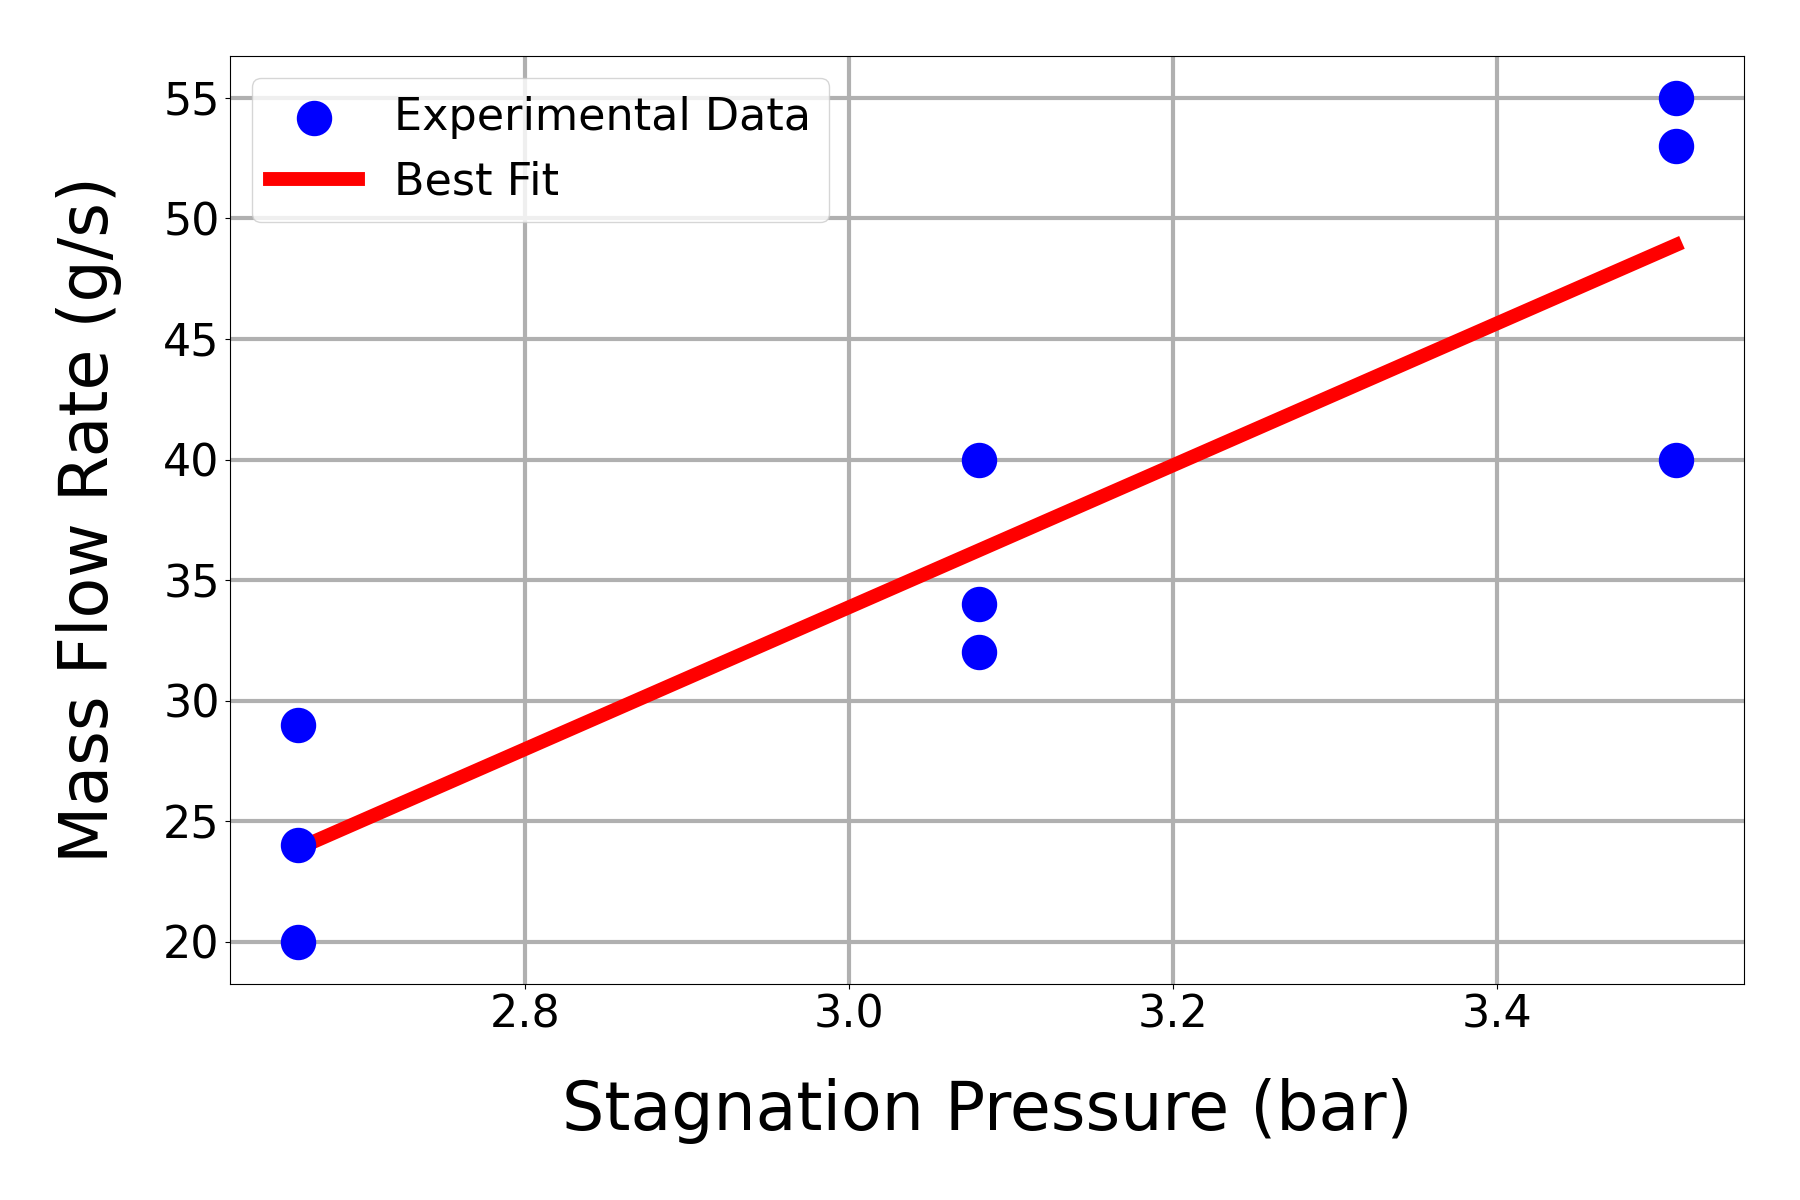
\includegraphics[width=\textwidth]{../report_assets/controllability_py.png}
        \caption{Mass Flow Rate Relationship with Stagnation Pressure}\label{fig:controllability-py}
    \end{minipage}    
\end{figure}    
While direct extrapolation to the lower flow rates reported in the literature would be inappropriate, the results nonetheless provide strong evidence that the required inlet pressure for powder feed systems can be significantly reduced. This is a parameter that has not been thoroughly investigated in prior studies, likely because feed systems for metallic powder-fed engines are designed to inject powder into combustion chambers operating at high pressures. In such systems, reducing a relative pressure difference between the tank inlet and outlet from 10 bar to 3 bar offers limited benefits, as the combustion chamber itself may be at pressures exceeding 30 bar. 

Although reducing the pressure rating of a 40 bar vessel to 33 bar yields some mass and volume savings, the impact is far more significant when reducing a 10 bar vessel to 3 bar. This makes the finding particularly valuable for ISM applications. In addition to the miniaturisation aspect, the required gas flow rate can be reduced. In space-based cold spray systems, gas is a non-renewable and limited resource. Therefore, lowering both the inlet pressure and the associated gas flow rate required for effective powder feeding provides clear advantages—specifically, reducing the quantity and pressure of gas that must be transported into space.


It should be noted, however, that the graph presented obscures an important detail: two distinct driving forces influence the mass flow rate, and these are non-trivially coupled. Therefore, further investigation into how these driving forces behave at lower pressures is required before this finding can be confidently used to inform design decisions.

\subsection{System Behaviour}
The system behaviour differed significantly from the expectations outlined in \autoref{sec:expected-behaviour}. As seen in \autoref{fig:real}, a fluidising region was observed in direct contact with the piston head, an unexpected result. 
\begin{figure}[htbp]
    \centering
    
    \begin{minipage}{0.6\textwidth}
        \centering
        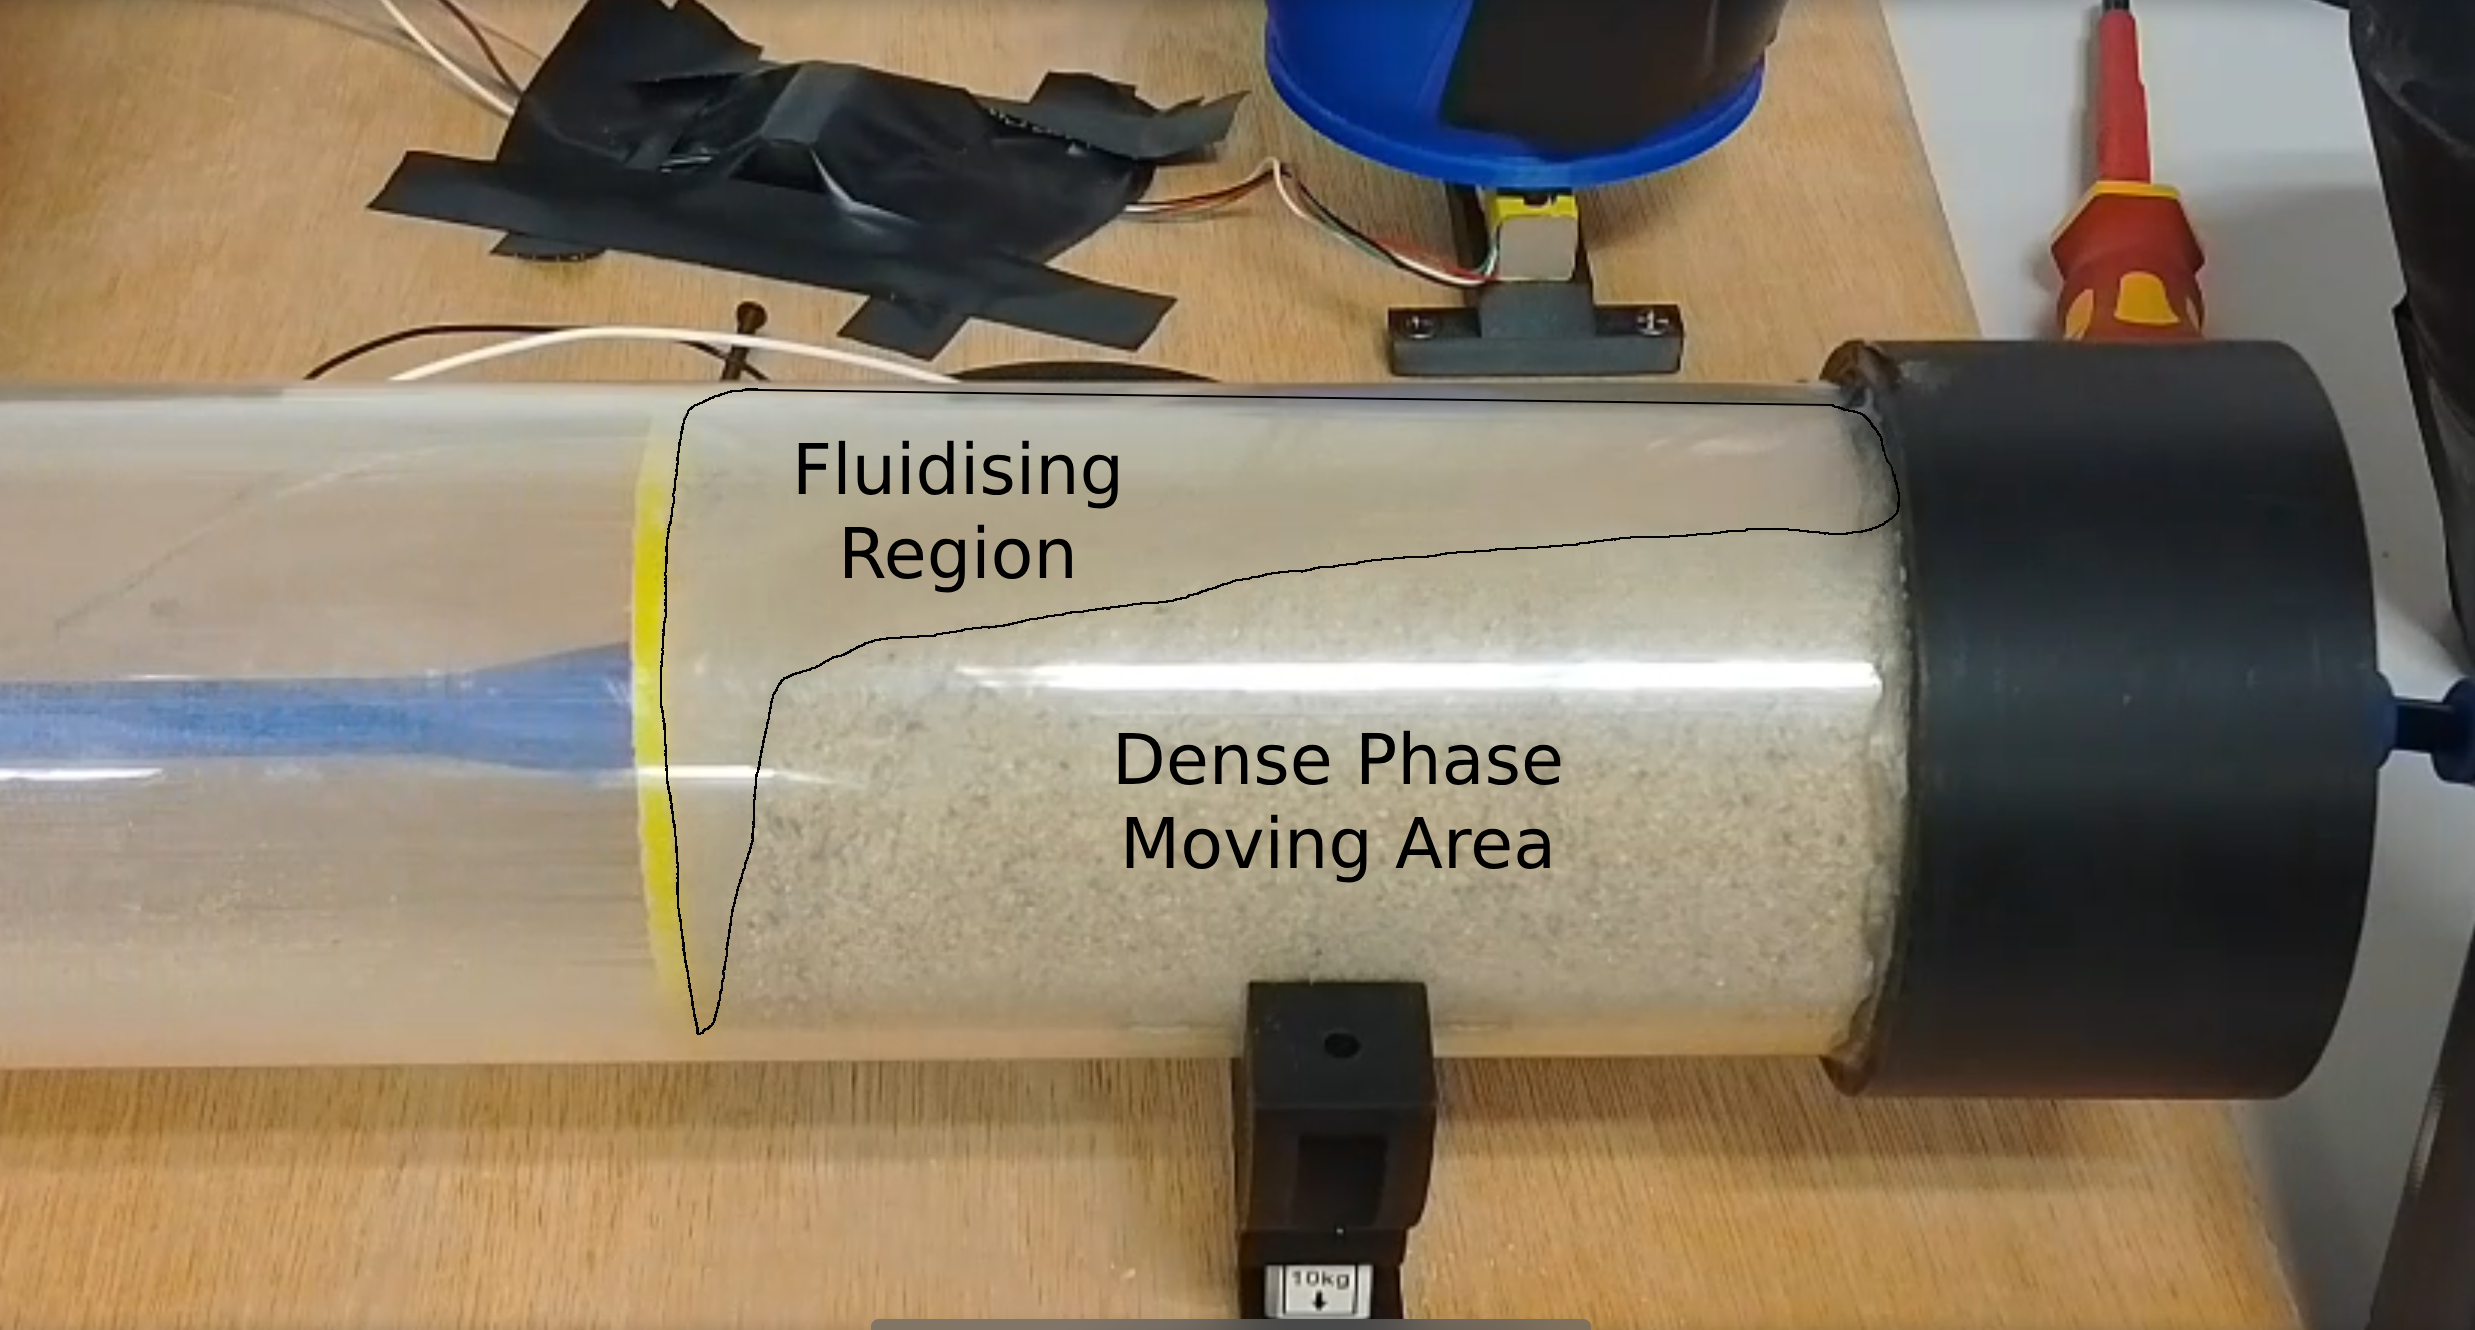
\includegraphics[width=\textwidth]{../report_assets/real_behaviour.png}
        \caption{A Snapshot of the 2nd 5 bar Inlet Test}\label{fig:real}
    \end{minipage}
    
\end{figure}
The end cap obstructs the view of the conical section, so it remains unclear whether a fluidising region was also present there, or whether the two regions may have been connected. It is hypothesised that this unexpected fluidisation pattern is due to the particle size of the powder. As discussed in \autoref{sec:background-powder-beds}, at the micron scale, gravity increasingly influences the fluidisation of larger particles. At the millimetre scale, gravitational effects may dominate entirely.

This behaviour was also accompanied by inconsistent piston movement, which progressed in discrete steps rather than with a smooth, continuous velocity. The cause of this behaviour is not well understood, and it is particularly surprising that it is not reflected in any of the mass flow rate data. It is possible that the powder was being rearranged inside the tank in discrete bursts while still being dispensed smoothly, or that redistribution occurred within the pipe as the powder travelled toward the separator. However, further analysis would be required to investigate this effect in detail.

\section{Numerical Analysis of Mass Flow Rate}
As mentioned in \autoref{sec:numerical-setup}, the validity of the simulations, especially given their 2D nature, are unknown. However the numerical investigation did present some potentially useful results.

\subsection{Results of System Under Microgravity}
The investigation into the flow under microgravity was conducted first and the simulation was tuned to this regime. The relationship between mass flow rate and piston velocity was conducted, recording the integration of the particle amount in the system over time as well as recording the particle distributions. As shown in \autoref{fig:sim-results-no-grav}, the relationship can be somewhat replicated as a positive correlation between mass flow and piston velocity can be seen.
\begin{figure}[htbp]
    \centering

    \begin{minipage}{0.45\textwidth}
        \centering
        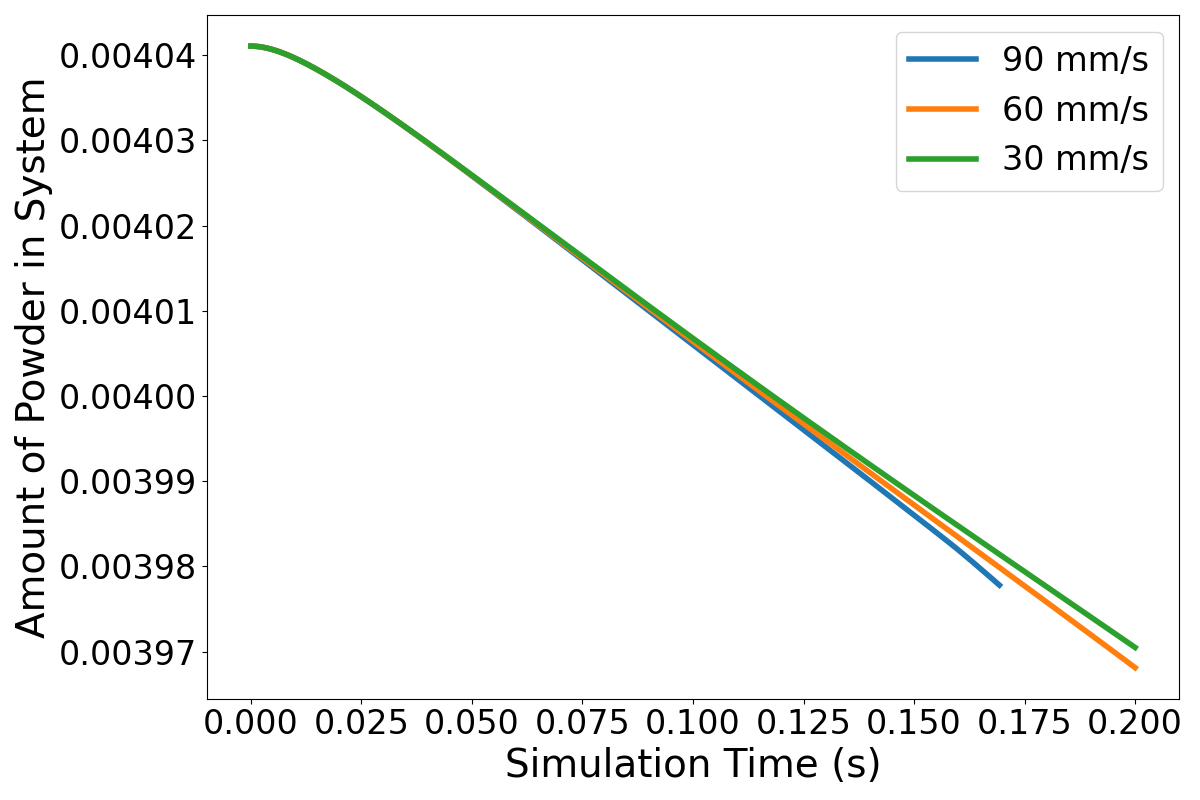
\includegraphics[width=\textwidth]{../report_assets/sim_no_grav_amount.png}
        \caption*{(a) Amount of Powder in the System}
    \end{minipage}    
    \hfill
    \begin{minipage}{0.45\textwidth}
        \centering
        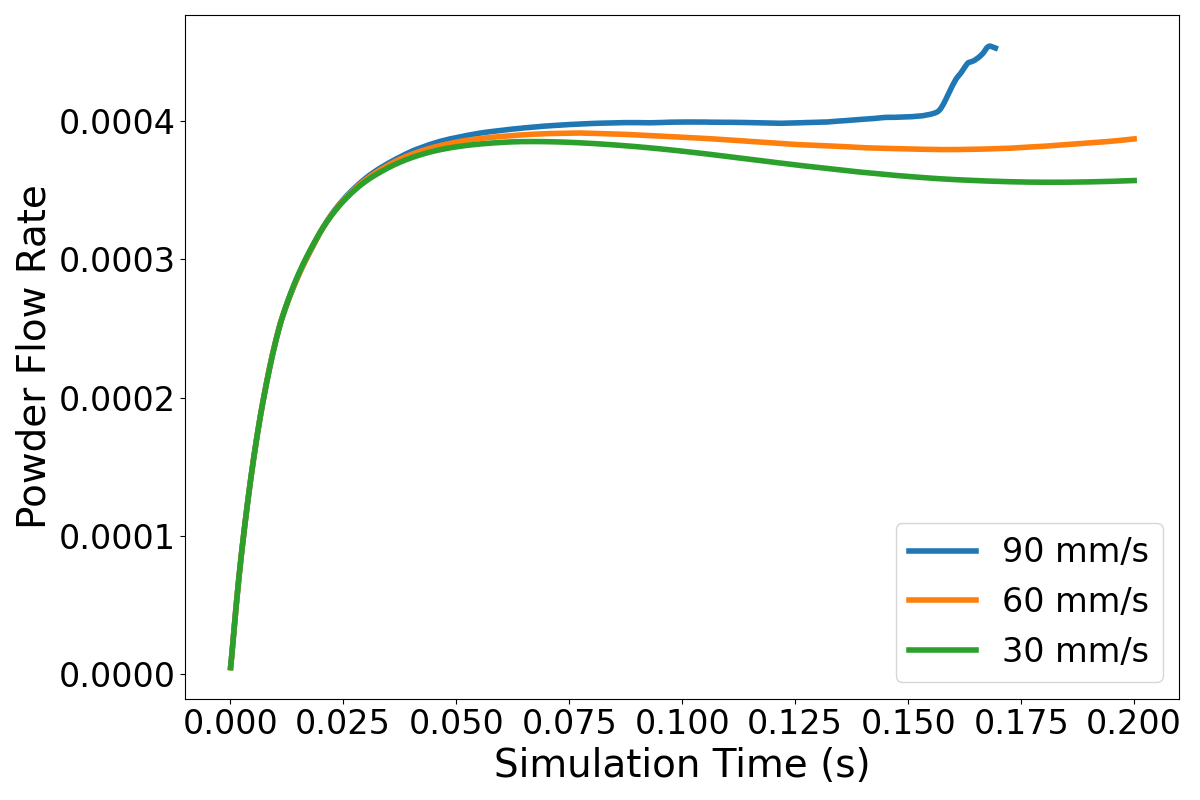
\includegraphics[width=\textwidth]{../report_assets/sim_no_grav_rate.png}
        \caption*{(b) Mass Flow Rate of Powder}
    \end{minipage}    
    \caption{Numerical Results of System Under Microgravity}\label{fig:sim-results-no-grav}

\end{figure} 
Interestingly, the powder mass flow rate initially starts at the same rate and only diverges after a time. Even then, it is not consistent, suggesting longer or more detailed simulations could reveal additional information.

The particle distributions at the start, 0.1s in and the end (whether that is 0.2 seconds for the successful simulations or 0.175 for the ones that crashed) are shown in \autoref{fig:30mm_no_grav} and \autoref{fig:90mm_no_grav}.
\begin{figure}[htbp]
    \centering

    \begin{minipage}{0.32\textwidth}
        \centering
        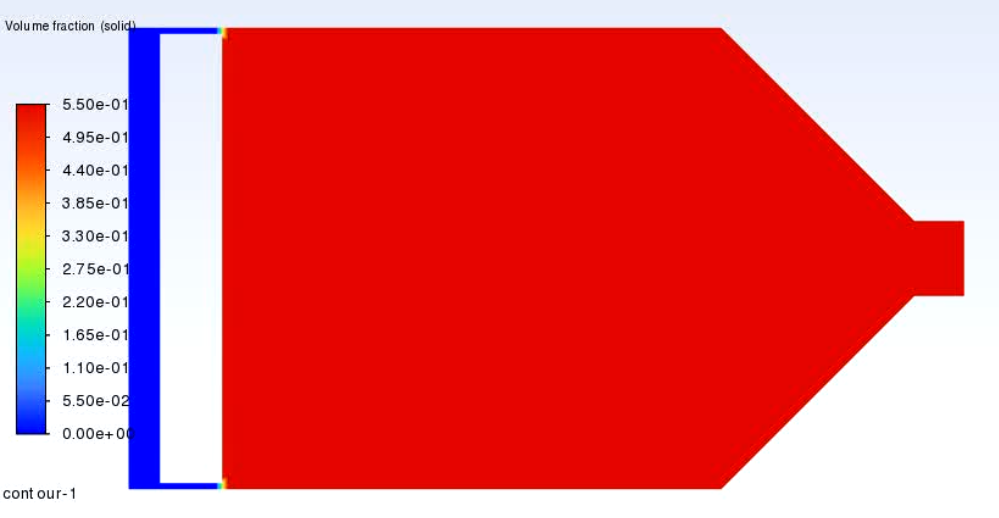
\includegraphics[width=\textwidth]{../report_assets/30mm_no_grav_1.png}
        \caption*{(a) Starting Distribution}
    \end{minipage}
    \hfill
    \begin{minipage}{0.32\textwidth}
        \centering
        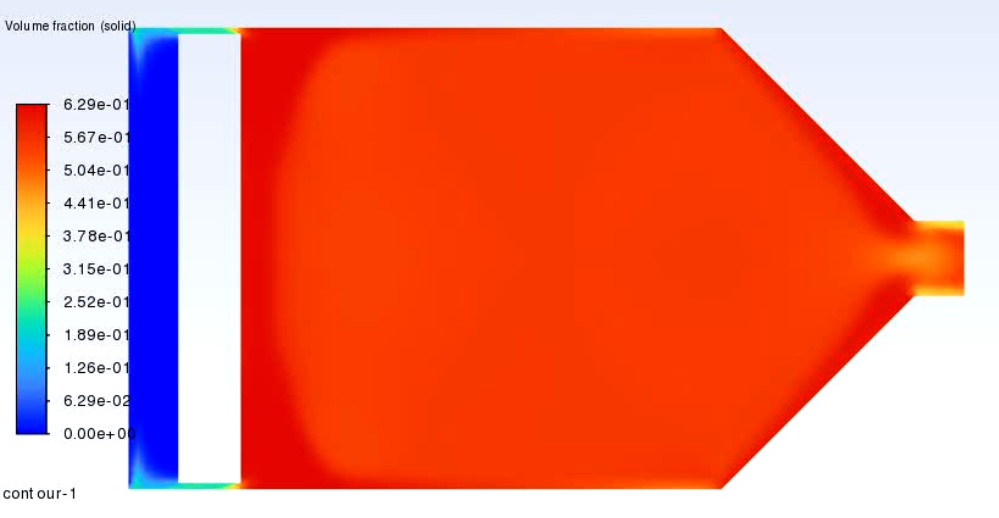
\includegraphics[width=\textwidth]{../report_assets/30mm_no_grav_2.png}
        \caption*{(b) Distribution after 0.1 seconds}
    \end{minipage}
    \hfill
    \begin{minipage}{0.32\textwidth}
        \centering
        \includegraphics[width=\textwidth]{../report_assets/30mm_no_grav_3.png}
        \caption*{(c) Final Distribution}
    \end{minipage}
    \caption{Particle Distributions from a Piston Velocity of 30 mm/s}

\end{figure}\label{fig:30mm_no_grav}

\begin{figure}[htbp]
    \centering

    \begin{minipage}{0.32\textwidth}
        \centering
        \includegraphics[width=\textwidth]{../report_assets/90mm_no_grav_1.png}
        \caption*{(a) Starting Distribution}
    \end{minipage}
    \hfill
    \begin{minipage}{0.32\textwidth}
        \centering
        \includegraphics[width=\textwidth]{../report_assets/90mm_no_grav_2.png}
        \caption*{(b) Distribution after 0.1 seconds}
    \end{minipage}
    \hfill
    \begin{minipage}{0.32\textwidth}
        \centering
        \includegraphics[width=\textwidth]{../report_assets/90mm_no_grav_3.png}
        \caption*{(c) Final Distribution}
    \end{minipage}
    \caption{Particle Distributions from a Piston Velocity of 90 mm/s}

\end{figure}\label{fig:90mm_no_grav}
These simulations seem to show two separate regions of particle density. While this could be viewed as supporting the theorised behaviour, outlined in \autoref{sec:expected-behaviour}, \autoref{fig:90mm_no_grav} (c) seems to suggest that when the piston moves fast enough towards the outlet, the fluidised region vanishes. This could be because the piston will move 90 mm/s in the simulation regardless of the force provided by any arching at the tube-cone interface or could be due to physics not captured by the chosen models, either way additional investigations into this could prove fruitful but were not conducted given the time requirements of the project.

\subsection{Results of System Under Earth's Gravity}
The simulations with gravity proved much more problematic. The ethos of the numerical investigation was to set up a system with identical parameters and only change the strength of gravitational force applied. This resulted in the system under gravity being relatively unrepresentative of the experimental phenomena observed. Shown in \autoref{fig:sim-results-grav}, the amount of powder in the system and the corresponding mass flow rate for the 30 mm/s and 90 mm/s piston velocities are shown.
\begin{figure}[htbp]
    \centering

    \begin{minipage}{0.45\textwidth}
        \centering
        \includegraphics[width=\textwidth]{../report_assets/sim_grav_amount.png}
        \caption*{(a) Amount of Powder in the System}
    \end{minipage}    
    \hfill
    \begin{minipage}{0.45\textwidth}
        \centering
        \includegraphics[width=\textwidth]{../report_assets/sim_grav_rate.png}
        \caption*{(b) Mass Flow Rate of Powder}
    \end{minipage}    
    \caption{Numerical Results of System Under Earth's Gravity}\label{fig:sim-results-grav}

\end{figure} 
Ideally, 60 mm/s would also have been investigated but given the troubleshooting of this behaviour took so long, there was no time to complete this set of studies. This independence of mass flow rate and piston velocity deviates from the literature and experimental results indicate an incorrect formulation of the simulation. The main cause for this is thought to be the value taken for the gravitational constant. Given nothing else to go off of, gravitational acceleration was taken to be 9.81 m/s. Considering the inlet velocity is 0.01 m/s, it is assumed that this was so large that it dominated the behaviour. As seen in \autoref{fig:30mm_grav} and \autoref{fig:90mm_grav}, the piston still increased compaction at the outlet with the void above the particles being much smaller in the 90 mm/s case.
\begin{figure}[htbp]
    \centering

    \begin{minipage}{0.32\textwidth}
        \centering
        \includegraphics[width=\textwidth]{../report_assets/30mm_grav_1.png}
        \caption*{(a) Starting Distribution}
    \end{minipage}
    \hfill
    \begin{minipage}{0.32\textwidth}
        \centering
        \includegraphics[width=\textwidth]{../report_assets/30mm_grav_2.png}
        \caption*{(b) Distribution after 0.1 seconds}
    \end{minipage}
    \hfill
    \begin{minipage}{0.32\textwidth}
        \centering
        \includegraphics[width=\textwidth]{../report_assets/30mm_grav_3.png}
        \caption*{(c) Mass Flow Rate}
    \end{minipage}
    \caption{Particle Distributions from a Piston Velocity of 30 mm/s}

\end{figure}\label{fig:30mm_grav}
\begin{figure}[htbp]
    \centering

    \begin{minipage}{0.32\textwidth}
        \centering
        \includegraphics[width=\textwidth]{../report_assets/90mm_grav_1.png}
        \caption*{(a) Starting Distribution}
    \end{minipage}
    \hfill
    \begin{minipage}{0.32\textwidth}
        \centering
        \includegraphics[width=\textwidth]{../report_assets/90mm_grav_2.png}
        \caption*{(b) Distribution after 0.1 seconds}
    \end{minipage}
    \hfill
    \begin{minipage}{0.32\textwidth}
        \centering
        \includegraphics[width=\textwidth]{../report_assets/90mm_grav_3.png}
        \caption*{(c) Mass Flow Rate}
    \end{minipage}
    \caption{Particle Distributions from a Piston Velocity of 90 mm/s}

\end{figure}\label{fig:90mm_grav}
However, there are no visual indications of fluidisation and therefore it is assumed that the velocity inlet is too little to promete it. Given more time, a new simulation would be setup, ideally in 3D to ground the inlet parameters and gravity in research-based values. 

Also of note, \autoref{fig:90mm_grav} (c) shows voids near the piston, right before crashing. This is thought to be a symptom of the deformed mesh issue discussed in \autoref{sec:numerical-setup}.
